\documentclass[symmetric,justified,marginals=raggedouter]{tufte-book}

%\hypersetup{colorlinks}% uncomment this line if you prefer colored hyperlinks (e.g., for onscreen viewing)

%%
% If they're installed, use Bergamo and Chantilly from www.fontsite.com.
% They're clones of Bembo and Gill Sans, respectively.
%\IfFileExists{bergamo.sty}{\usepackage[osf]{bergamo}}{}% Bembo
%\IfFileExists{chantill.sty}{\usepackage{chantill}}{}% Gill Sans

%\usepackage{microtype}

%%
% For nicely typeset tabular material
\usepackage{booktabs}

%%
% For graphics / images
\usepackage{graphicx}
\setkeys{Gin}{width=\linewidth,totalheight=\textheight,keepaspectratio}
\graphicspath{{graphics/}}

% The fancyvrb package lets us customize the formatting of verbatim
% environments.  We use a slightly smaller font.
\usepackage{fancyvrb}
\fvset{fontsize=\normalsize}

%%
% Prints argument within hanging parentheses (i.e., parentheses that take
% up no horizontal space).  Useful in tabular environments.
\newcommand{\hangp}[1]{\makebox[0pt][r]{(}#1\makebox[0pt][l]{)}}

%%
% Prints an asterisk that takes up no horizontal space.
% Useful in tabular environments.
\newcommand{\hangstar}{\makebox[0pt][l]{*}}

%%
% Prints a trailing space in a smart way.
\usepackage{xspace}

%%
% Some shortcuts for Tufte's book titles.  The lowercase commands will
% produce the initials of the book title in italics.  The all-caps commands
% will print out the full title of the book in italics.
\newcommand{\vdqi}{\textit{VDQI}\xspace}
\newcommand{\ei}{\textit{EI}\xspace}
\newcommand{\ve}{\textit{VE}\xspace}
\newcommand{\be}{\textit{BE}\xspace}
\newcommand{\VDQI}{\textit{The Visual Display of Quantitative Information}\xspace}
\newcommand{\EI}{\textit{Envisioning Information}\xspace}
\newcommand{\VE}{\textit{Visual Explanations}\xspace}
\newcommand{\BE}{\textit{Beautiful Evidence}\xspace}

\newcommand{\TL}{Tufte-\LaTeX\xspace}

% Prints the month name (e.g., January) and the year (e.g., 2008)
\newcommand{\monthyear}{%
  \ifcase\month\or January\or February\or March\or April\or May\or June\or
  July\or August\or September\or October\or November\or
  December\fi\space\number\year
}


% Prints an epigraph and speaker in sans serif, all-caps type.
\newcommand{\openepigraph}[2]{%
  %\sffamily\fontsize{14}{16}\selectfont
  \begin{fullwidth}
  \sffamily\large
  \begin{doublespace}
  \noindent\allcaps{#1}\\% epigraph
  \noindent\allcaps{#2}% author
  \end{doublespace}
  \end{fullwidth}
}

% Inserts a blank page
\newcommand{\blankpage}{\newpage\hbox{}\thispagestyle{empty}\newpage}

\usepackage{units}

% Typesets the font size, leading, and measure in the form of 10/12x26 pc.
\newcommand{\measure}[3]{#1/#2$\times$\unit[#3]{pc}}

% Macros for typesetting the documentation
\newcommand{\hlred}[1]{\textcolor{Maroon}{#1}}% prints in red
\newcommand{\hangleft}[1]{\makebox[0pt][r]{#1}}
\newcommand{\hairsp}{\hspace{1pt}}% hair space
\newcommand{\hquad}{\hskip0.5em\relax}% half quad space
\newcommand{\TODO}{\textcolor{red}{\bf TODO!}\xspace}
\newcommand{\ie}{\textit{i.\hairsp{}e.}\xspace}
\newcommand{\eg}{\textit{e.\hairsp{}g.}\xspace}
\newcommand{\na}{\quad--}% used in tables for N/A cells
\providecommand{\XeLaTeX}{X\lower.5ex\hbox{\kern-0.15em\reflectbox{E}}\kern-0.1em\LaTeX}
\newcommand{\tXeLaTeX}{\XeLaTeX\index{XeLaTeX@\protect\XeLaTeX}}
% \index{\texttt{\textbackslash xyz}@\hangleft{\texttt{\textbackslash}}\texttt{xyz}}
\newcommand{\tuftebs}{\symbol{'134}}% a backslash in tt type in OT1/T1
\newcommand{\doccmdnoindex}[2][]{\texttt{\tuftebs#2}}% command name -- adds backslash automatically (and doesn't add cmd to the index)
\newcommand{\doccmddef}[2][]{%
  \hlred{\texttt{\tuftebs#2}}\label{cmd:#2}%
  \ifthenelse{\isempty{#1}}%
    {% add the command to the index
      \index{#2 command@\protect\hangleft{\texttt{\tuftebs}}\texttt{#2}}% command name
    }%
    {% add the command and package to the index
      \index{#2 command@\protect\hangleft{\texttt{\tuftebs}}\texttt{#2} (\texttt{#1} package)}% command name
      \index{#1 package@\texttt{#1} package}\index{packages!#1@\texttt{#1}}% package name
    }%
}% command name -- adds backslash automatically
\newcommand{\doccmd}[2][]{%
  \texttt{\tuftebs#2}%
  \ifthenelse{\isempty{#1}}%
    {% add the command to the index
      \index{#2 command@\protect\hangleft{\texttt{\tuftebs}}\texttt{#2}}% command name
    }%
    {% add the command and package to the index
      \index{#2 command@\protect\hangleft{\texttt{\tuftebs}}\texttt{#2} (\texttt{#1} package)}% command name
      \index{#1 package@\texttt{#1} package}\index{packages!#1@\texttt{#1}}% package name
    }%
}% command name -- adds backslash automatically
\newcommand{\docopt}[1]{\ensuremath{\langle}\textrm{\textit{#1}}\ensuremath{\rangle}}% optional command argument
\newcommand{\docarg}[1]{\textrm{\textit{#1}}}% (required) command argument
\newenvironment{docspec}{\begin{quotation}\ttfamily\parskip0pt\parindent0pt\ignorespaces}{\end{quotation}}% command specification environment
\newcommand{\docenv}[1]{\texttt{#1}\index{#1 environment@\texttt{#1} environment}\index{environments!#1@\texttt{#1}}}% environment name
\newcommand{\docenvdef}[1]{\hlred{\texttt{#1}}\label{env:#1}\index{#1 environment@\texttt{#1} environment}\index{environments!#1@\texttt{#1}}}% environment name
\newcommand{\docpkg}[1]{\texttt{#1}\index{#1 package@\texttt{#1} package}\index{packages!#1@\texttt{#1}}}% package name
\newcommand{\doccls}[1]{\texttt{#1}}% document class name
\newcommand{\docclsopt}[1]{\texttt{#1}\index{#1 class option@\texttt{#1} class option}\index{class options!#1@\texttt{#1}}}% document class option name
\newcommand{\docclsoptdef}[1]{\hlred{\texttt{#1}}\label{clsopt:#1}\index{#1 class option@\texttt{#1} class option}\index{class options!#1@\texttt{#1}}}% document class option name defined
\newcommand{\docmsg}[2]{\bigskip\begin{fullwidth}\noindent\ttfamily#1\end{fullwidth}\medskip\par\noindent#2}
\newcommand{\docfilehook}[2]{\texttt{#1}\index{file hooks!#2}\index{#1@\texttt{#1}}}
\newcommand{\doccounter}[1]{\texttt{#1}\index{#1 counter@\texttt{#1} counter}}

% Generates the index
\usepackage{makeidx}
\makeindex


\usepackage{indentfirst}

\usepackage[utf8]{inputenc}
\usepackage[T1]{fontenc}

%%%%%%%%%%%%%%%%%%%%%%%%%%%%%%%% Customization %%%%%%%%%%%%%%%%%%%%%%%%%%%%%%%%

\setcounter{tocdepth}{1}
\setcounter{secnumdepth}{1}

\renewcommand\contentsname{\normalfont \huge Table des matières}

\titlecontents{chapter}%
    [0em]% distance from left margin
    {\vspace{1\baselineskip}\begin{fullwidth}Chapitre }% above (global formatting of entry)
    {\contentslabel{0em} \hspace{1em} \huge $\vert$ \Large}% before w/ label (label = ``Chapter 1'')
    {\hspace{1em}}% before w/o label
    {\hfill\qquad\thecontentspage}% filler and page (leaders and page num)
    [\end{fullwidth}]% after
\titlecontents{section}% FIXME
    [0em] % distance from left margin
    {\vspace{0\baselineskip}\begin{fullwidth} \rmfamily\itshape} % above (global formatting of entry)
    {\hspace*{6em}\contentslabel{2em}} % before w/label (label = ``2.6'')
    {\hspace*{7em}} % before w/o label
    {\normalfont\hfill\qquad\thecontentspage} % filler + page (leaders and page num)
    [\end{fullwidth}] % after

\usepackage{enumitem}
\setlist{leftmargin=20mm}

\usepackage{tikz}
\usetikzlibrary{calc}

\newcommand\tikzmark[1]{%
  \tikz[overlay,remember picture] \coordinate (#1);}
  
 \renewcommand\labelitemi{--}

\usepackage{multirow}

\makeatletter
    \newcommand{\vast}{\bBigg@{3}}
    \newcommand{\Vast}{\bBigg@{3.5}}
    \newcommand{\vastt}{\bBigg@{4}}
    \newcommand{\Vastt}{\bBigg@{11}}
    %%
    %% Size from smallest to largest:
    %%\[ ( \big( \Big( \bigg( \Bigg( \vast( \Vast( \vastt( \Vastt(\]
\makeatother

\begin{document}

% Front matter
\frontmatter

%%%%%%%%%%%%%%%%%%%%%%%%%%%%%%%%%%%% Titre %%%%%%%%%%%%%%%%%%%%%%%%%%%%%%%%%%%%

\newpage
\author{Quentin Lobbé}
\title{\nohyphenation{Archives et Fragments Web}}
\cleardoublepage
{  
  \begin{fullwidth}%
  \thispagestyle{empty} 
  \setlength{\parskip}{\baselineskip}
  \begingroup
  \vspace*{10em}
  \par\noindent\Large{Quentin Lobbé}
  \vspace*{-1em}
  \par\noindent\Huge\textbf{Archives et Fragments Web}
  \par\noindent\nohyphenation\Large{Désagréger les archives Web pour mener une exploration temporelle de traces numériques des migrations}
  \endgroup
  \vfill  
  \par\noindent\nohyphenation Université Paris-Saclay, École doctorale des sciences et technologies de l'information et de la communication.  Thèse pour l'obtention du doctorat de Télécom ParisTech et de l'Université Paris-Saclay.    
  \end{fullwidth}%
}

\blankpage

%%%%%%%%%%%%%%%%%%%%%%%%%%%%%%%%%%%% Info Thèse %%%%%%%%%%%%%%%%%%%%%%%%%%%%%%%%%%%%
  
\newpage
\begin{fullwidth}
~\vfill
\thispagestyle{empty}
\setlength{\parskip}{\baselineskip}

\par\noindent Thèse présentée par \textbf{\thanklessauthor}\\
LTCI, Télécom ParisTech, Université Paris Saclay \& Inria. Paris, France.\\
quentin.lobbe@telecom-paristech.fr

\par\noindent Sous la direction de :\\
\textbf{Pierre Senellart}, professeur à l'École Normale Supérieure\\
\textbf{Dana Diminescu}, professeure à Télécom ParisTech

\par\noindent Soutenue publiquement à Paris le 9 novembre 2018, devant un jury composé de :\\
\textbf{Bruno Bachimont} (Rapporteur), enseignant-chercheur à l'Université Technologique de Compiègne\\
\textbf{Marc Spaniol} (Rapporteur), professeur à l'Université de Caen Basse-Normandie\\
\textbf{Anat Ben-David}, professeure à l'Open University of Israel\\
\textbf{Dominique Cardon}, professeur associé à Sciences Po Paris\\
\textbf{Bruno Defude}, directeur adjoint de la recherche et des formations doctorales à Télécom SudParis

\par\textit{last modified \monthyear}
\end{fullwidth}
  
\thispagestyle{empty}%
\clearpage%

%%%%%%%%%%%%%%%%%%%%%%%%%%%%%%%% Remerciements %%%%%%%%%%%%%%%%%%%%%%%%%%%%%%%%

\newpage

~\vfill
\noindent
\par\noindent Il me demanda de chercher la première page.\\
\noindent Je posais ma main gauche sur la couverture et ouvris le volume de mon pouce serré contre l'index. Je m'efforçais en vain : il restait toujours des feuilles entre la couverture et mon pouce. Elles semblaient sourdre du livre.\\
- Maintenant cherchez la dernière.\\
\noindent Mes tentatives échouèrent de même; à peine pus-je balbutier d'une voix qui n'était plus ma voix :\\
- Cela n'est pas possible.\\
\noindent Toujours à voix basse le vendeur me dit : \\
- Cela n'est pas possible et pourtant cela \textit{est}. Le nombre de pages de ce livre est exactement infini. Aucune n'est la première, aucune n'est la dernière.
\\~\\
\noindent\textit{Jorge Luis Borges - Le livre de sable} 
\vfill
\indent
\newpage
\begingroup
\vspace*{8em}
\huge $\vert$ \huge Remerciements
\vspace*{4em}
\par\normalsize Ici je remercie plein de gens

\par Beaucoup de gens

\par Mais vraiment
\endgroup
\vfill

%%%%%%%%%%%%%%%%%%%%%%%%%%%%%%%%%%%% Tables %%%%%%%%%%%%%%%%%%%%%%%%%%%%%%%%%%%%

\tableofcontents

\listoffigures

\listoftables

\mainmatter

%%%%%%%%%%%%%%%%%%%%%%%%%%%%%%%%%% Chapitre 1 %%%%%%%%%%%%%%%%%%%%%%%%%%%%%%%%%%

\chapter{Introduction}

\section{Introduction générale}

Ici l'intro de la thèse.

\section{Mise en garde}

\subsection{Penser le passé depuis le présent}

Ici on fait un rapide détour par l'historiographie et les difficultés à parler du passé depuis le présent.

\subsection{Conservation différentielle et nature des archives Web}

Ici on parle de la raréfaction de la matière Web à mesure que l'on remonte le temps et également à mesure que le web fournit du contenu.

%%%%%%%%%%%%%%%%%%%%%%%%%%%%%%%%%% Chapitre 2 %%%%%%%%%%%%%%%%%%%%%%%%%%%%%%%%%%

\chapter{Du Web aux Représentations en Ligne des Diasporas}
\label{chap:2}

\section{Retour aux origines du Web}
\label{sec:2_web}

\section{Le migrant connecté}

\section{Le Web, espace de communication et d'organisation}

The Web is the main publishing application of the Internet.
As such, it consists mainly of the combination of three standards, the URI (Berners-Lee 1994) defining a naming space for object on the Internet, 6 HTTP (Fielding et al. 1999) defining a client–server interaction protocol using hyperlinks at its core, and HTML (Berners-Lee and Connolly 1995) an SGML DTD that defines the layout rendering of pages in browsers.
The implementation of these three standards enables any computer connected to the Internet to be- come a publishing system.

But the fact that it is actionable on the Web changes the way references are used by fragmenting content to smaller addressable pieces and overall favoring transversal navigation and access to content which in return, deeply changes the nature of writing as well as reading (Aarseth 1997; Landow 1997; Bolter 2001).

Géopolitique de l'hypertexte

Le web est un digital cultural artifact (Lyman and Kahle 1998)

 the Web does, to a large extend, re-use previous forms of publishing 12 (Crowston and Williams 1997; Eriksen and Ihlström 2000; Shepherd and Polanyi 2000), it also invents new ones.
 
This characterization of the Web as a distributed hypermedia openly and permanently authored at a global scale entails that Web archiving can only achieve preservation of limited aspects of a larger and living cultural artifact.

the interconnectedness of content is a major quality of the Web that raises issues when it comes to archiving.

\section{L'Atlas e-Diasporas}
\label{sec:2_atlas}

%%%%%%%%%%%%%%%%%%%%%%%%%%%%%%%%%% Chapitre 3 %%%%%%%%%%%%%%%%%%%%%%%%%%%%%%%%%%

\chapter{Archiver le Web}

\noindent Face à la disparition totale ou partielle des sites Web recensés par l'atlas e-Diasporas (Chapitre \ref{chap:2}), il a été décidé de lancer une campagne d'archivage afin de préserver cet héritage numérique et d'anticiper, par là même, la tenue de futures recherches. Sans cette initiative, mes travaux de thèse n'auraient pas pu exploiter et questionner les traces d'un Web aujourd'hui passé. 

De part la nature même du médium, le Web demande de penser et de mettre en place un archivage particulier, basé sur des techniques de collectage dédiées. Dans ce chapitre, nous évoquerons la genèse de l'archivage du Web qui, au tournant des années 2000, a connu un essor mondial, mobilisant nombre d'acteurs et d'institutions. Nous introduirons ensuite, d'un point de vue technique, les principales méthodes de sélection, collecte et stockage des corpus à archiver. Nous présenterons enfin les contours des archives e-Diasporas à proprement parler. Ses particularités et ses caractéristiques. Sa durée et son étendue. \\

\noindent Bien que cette thèse se concentre sur l'exploration d'archives Web déjà existantes, il nous semble important d'évoquer la façon dont ces dernières sont constituées en amont afin de mieux saisir les biais analytiques (Chapitre \ref{chap:4}) qui motiveront la présentation de notre principale contribution (Chapitre \ref{chap:5}). Ce faisant, les éléments que nous nous apprêtons à présenter s'appuieront principalement sur l'ouvrage de J.~Masanes : "\textit{Web Archiving}" \citep{masanes_web_2006} qui reste encore aujourd'hui une référence.

\section{Vingt ans d'archivage du Web}
\label{sec:3_20ans}

\noindent En Octobre 2016, se tenait à la Bibliothèque Nationale de France (BNF) une grande conférence anniversaire réunissant, pour les 20 ans de l'archivage du Web\footnote{\url{http://www.bnf.fr/fr/professionnels/anx_journees_pro_2016/a.jp_161122_23_archivage_web.html}}, les acteurs français de la pratique. Alors qu'était évoqués les conditions du partage du dépôt légal du Web national entre la BNF et l'INA, il a été rappelé qu'à l'origine chacune des deux institutions souhaitait se voir attribuer la pleine gestion de ce dépôt. L'INA mettait en avant ses compétences techniques acquises en archivant les flux audiovisuels nouvellement introduits dans le paysage culturel. La BNF, pour sa part, s'appuyait sur son expérience pluricentenaire de préservation du patrimoine\footnote{\url{http://multimedia.bnf.fr/video/prof/161123_10_dl_web.mp4}}. 

Cette querelle initiale et son dénouement (la cotutelle du dépôt légale) sont à l'image de l'histoire même de l'archivage du Web: la conjugaison d'une tradition longue de sauvegarde des savoirs et d'un ensemble de techniques de collecte nouvellement pensées pour cet objet complexe qu'est le Web, le tout porté par une poignée de pionniers.

\subsection{Préserver la mémoire collective}

\noindent L'archivage du Web s'inscrit dans la tradition longue des techniques d'élaboration et de conservation de la mémoire collective. Tradition qui remonte aux origines même de l'humanité où technique et mémoire se trouvaient étroitement liées. 

A. Leroi-Gourhan fait émerger, de l'étude de séries d'objets (silex taillés, percuteurs, harpons, etc) et de figures préhistoriques (gravures et peintures des grottes ornées), une ligne de rencontre entre technique et mémoire \citep{leroi-gourhan_geste_1964}. Le préhistorien décrit la technique comme un système évolutif, soumis aux lois générales de la technologie et apparaissant comme transversal à des cultures parfois diverses et éloignées\footnote{
Leroi-Gourhan associe les formes animales des grottes ornées à des signes, réalisant des couplages basés sur l'observation (comptages et statistiques) de dizaines de cavités. Il cherche à établir une échelle évolutive des styles pariétaux, transversale aux premiers âges de l'Europe de l'Ouest \citep{leroi-gourham_art_1984}}. La technique est chargée, en elle même, de l'histoire passée des continuités, ruptures et transformations technologiques dont elle est l'aboutissement à un instant t.   

Avec Leroi-Gourhan, la technique devient mémoire. Elle peut en être chargée et/ou être conçue à dessein de la conserver. Involontairement, le silex taillé porte en lui la trace de l'homme qui l'a élaboré. Lorsque le tailleur finit par mourir, son geste continue à s'extérioriser à travers l'outil qui demeure. Précieux indice pour celui qui vient à sa suite ou pour l'archéologue qui, des millénaires après, saura grâce à cet objet assembler les traces fragmentées d'une pratique passée. Mais l'homme aurait aussi très bien pu choisir, en conscience, d'inscrire son expérience individuelle sur des supports de mémoire dédiés. L'écriture est ainsi l'une des premières techniques de la mémoire, utilisée par l'humanité depuis le néolithique. L'écriture est en cela une \textit{mnémotechnologie} \citep{stiegler_leroi-gourhan:_1998}. 

Poursuivant son évolution, l'humanité développe plus avant les techniques de transmission des savoirs pour sélectionner et agréger ses expériences individuelles en une mémoire collective. Des espaces et des structures voient le jour, appuyés par divers pouvoirs politiques ou religieux, avec le double objectif de préserver et d'administrer l'héritage collectif. J. Derrida décrit ainsi le geste d'archiver comme un "\textit{geste de pouvoir}" \citep{derrida_trace_2014}. Choisir ce que l'on garde ou non dans les archives ne peut être que le fruit d'une hégémonie, d'une hiérarchie et "\textit{d'un certain nombre d'opérations de pouvoir}" rendues légitimes par une institution. L'État est ainsi caractérisé par \textit{sa capacité d'accumuler, contrôler et exploiter la mémoire collective} \citep{stiegler_etat_1991}, capacité dont on retrouve divers incarnations au court de l'histoire :

\begin{itemize}[leftmargin=*]  
\item Au IVe millénaire av. J.C, les tablettes d'argiles étaient accumulées par les mésopotamiens pour constituer les premières bibliothèques
\item Entre 535 et 555, Cassiodore pense le Monastère de Vivarium comme un lieu de transmission où, pour la première fois, seraient associés culture savante et christianisme
\item François Ier crée le dépôt légal\footnote{"\textit{Nous avons délibéré de faire retirer, mettre et assembler en notre librairie toutes les livres dignes d'être vues qui ont été ou qui seront faites, compilées, amplifiées, corrigées et amendées de notre tems}", extrait de l'ordonnance royale \citep{dougnac_depot_1960}} en France, par l'ordonnance royale du 28 décembre 1537, à des fins de préservation culturelle mais également de contrôle politique
\end{itemize}

\noindent Les siècle passent et les archives s'adaptent à la transformation des supports de mémoire et à l'émergence de formes nouvelles d'enre\-gistrement. Avec l'arrivée des technologies analogiques\footnote{Cinématographie, photographie, radiodiffusion, etc}, il faut désormais capter et archiver des flux d'images et de sons, ce qui conduira en France à la création de l'Institut National de l'Audiovisuel (INA) en 1974. L'apparition du numérique\footnote{Bases de données, logiciels, interfaces, etc} marque la dernière étape de ce cheminement en ouvrant la voie à un renouveau des formes de lecture et d'étude des archives. L'accès à distance de documents numérisés facilite leur consultation, mais il devient également possible de les qualifier, de les annoter ou de les mettre en relation, et ce, de manière large voire exhaustive \citep{borgman_digital_2000} :

\begin{itemize}[leftmargin=*]  
\item En 1971, le projet Gutenberg commence à collecter des copies numéri\-ques (recopiées et tapées \textit{à la main}) d'ouvrages du domaine public
\item Le Thesaurus Linguae Graecae cherche, depuis 1972, à numériser la plupart des textes littéraires rédigés en grecs ancien et toujours subsistants
\end{itemize}

\noindent Mais si le numérique permet aujourd'hui de revisiter des ressources anciennement archivées, il est aussi créateur d'objets nativement numé\-riques tout autant porteurs d'un héritage à préserver. Le web en est la parfaite illustration.

\subsection{Un héritage numérique}

\noindent L'archivage du Web débute à la fin des années 90, et plus précisément en 1996 lorsque se développent les premières initiatives de préservation du Web, soit 4 années à peine après la publication de la première page sur la toile~(Section \ref{sec:2_web}). La National Library of Australia est ainsi à l'initiative du projet Pandora\footnote{\url{http://pandora.nla.gov.au/}} qui vise à archiver les publications en ligne australiennes sur la base d'une collecte sélective et continue de sites Web australiens. La Swedish Royal Library, quant à elle, lance le projet Kulturarw3\footnote{\url{https://web.archive.org/web/20040206225053/https://www.kb.se/kw3}} qui s'essaye à une collecte "\textit{intégrale}" et espacée dans le temps des sites du Web suédois \citep{arvidson_kulturarw3_2000}.

Mais c'est avec la création d'Internet Archive par B. Kahle la même année \citep{kahle_preserving_1997}, que s'écrit véritablement la première page de l'histoire des archives du Web. Ingénieur et activiste, Kahle s'inspire de la Bibliothèque d'Alexandrie pour motiver la création d'une organisation à but non lucratif afin de rendre accessible au plus grand nombre le passé du Web\footnote{\url{https://archive.org/}}. Utilisant un crawler développé pour le compte de son autre société Alexa Internet, Kahle revendiquait, dans les premières années de la collecte, être capable d'archiver au moins une fois tous les deux mois chacun des sites de l'ensemble du Web \citep{mohr_introduction_2004}. La revente d'Alexa au groupe Amazon en 1999 va lui permettre de pérenniser financièrement Internet Archive, qui depuis ce temps n'a eu de cesse d'archiver le Web.

Ces pionniers de l'archivage sont rapidement suivis par la Finlande en 1997, le Danemark en 1998 et d'autres pays nordiques rassemblés autour du projet NWA\footnote{Nordic Web Archive} \citep{hallgrinsson_nordic_2003}. En 2003, la publication par l'UNESCO de la \textit{Charte sur la conservation du patrimoine numérique} \citep{unesco_charter_2003} marque un nouveau tournant pour l'archivage du Web en reconnaissant la valeur universelle d'une telle démarche et l'urgence face à la disparition potentiel de tout, ou d'une partie, de l'héritage numérique mondial : \\

\begin{fullwidth}
"\textit{Le  patrimoine  numérique  mondial  risque  d'être  perdu  pour  la  postérité.  Les  facteurs  qui  peuvent  contribuer  à  sa  perte  sont  l'obsolescence  rapide  du  matériel  et  des  logiciels  qui  servent  à  le  créer,  les  incertitudes  concernant  les  financements,  la  responsabilité  et  les  méthodes  de  la  maintenance  et  de  la  conservation et l'absence de législation favorable à sa préservation. L'évolution des attitudes n'a pas suivi celle des technologies. L'évolution numérique a été trop rapide et trop coûteuse pour que les pouvoirs publics et les institutions élaborent en temps voulu et en connaissance de cause des stratégies de conservation. La menace qui plane sur le potentiel économique, social, intellectuel et culturel du patrimoine, pierre angulaire de l'avenir, n'a pas été pleinement saisie.}" 

\noindent(Charte sur la conservation du patrimoine numérique, Article 3)\\
\end{fullwidth}

\noindent Pour de nombreuses bibliothèques nationales, la charte de l'UNESCO fait l'effet d'un accélérateur (Figure \ref{fig:date-initiative}). Les institutions sont encouragées dès 2003 à archiver leur Web national \citep{gomes_survey_2011}. Mais notons ici que la notion de Web national reste discutable \citep{abiteboul_first_2002}, il s'agira souvent de crawler le Web en fonction d'une extension de nom de domaine donnée (.fr, .jp, .uk, etc), extension qui ne couvre pas exhaustivement l'ensemble des sites associés à un domaine national précis, elle est plutôt à considérer comme une borne inférieure de celui-ci \citep{koehler_analysis_1999}. Le cas des corpus de l'Atlas e-Diasporas en est un très bon contre-exemple, nombre de sites migrants possédant une extension générique (.com, .net) ou correspondant au pays d'accueil plutôt qu'au pays d'origine \citep{leclerc_cyberespace_2012}.  

\begin{figure}%
  \includegraphics[width=\linewidth]{graphics/date-initiative}
  \caption{Évolution cumulée du nombre d'initiatives d'archivage du Web par année de création (source de données \citep{gomes_survey_2011} et Wikipédia \url{https://en.wikipedia.org/wiki/List_of_Web_archiving_initiatives})}
  \label{fig:date-initiative}
\end{figure} 

\noindent Ces nouveaux acteurs de l'archivage du Web peuvent être classés suivant la terminologie introduite par J. Masanes \citep{masanes_web_2006}, entre initiatives publiques ou privées, poursuivant un but lucratif ou non. L'accès aux corpus archivés peut être entièrement public ou restreint et limité, en ligne ou physique (machine de consultation dans une bibliothèque). Par exemple, Internet Archive est une initiative à but non lucratif, avec un accès public à l'ensemble de ses corpus, en ligne depuis 2001 et physique depuis 2002\footnote{La Wayback Machine est officiellement lancée en 2001. Avant cette date les corpus d'Internet Archives n'étaient pas accessibles au public. En 2002, une copie intégrale des archives est consultable à la Bibliotheca Alexandrina, en Égypte}. 

Une autre manière de catégoriser ces initiatives est de regarder la nature des corpus archivés. Nous avons déjà évoqué les corpus territoriaux censés capturer les contours d'un Web national. Cette notion peut être également transposée à plus fine échelle : celle d'une région ou d'une ville \citep{boudrez_archiving_2002}. Un corpus d'archive peut être conçu pour cibler une thématique donnée, souvent  centrée sur des événements politiques \citep{voerman_archiving_2002,schneider_building_2003} : élections, référendums, etc. Certaines initiatives s'affranchissent même de barrières géographiques devenues contraignantes en préservant des sites de domaines nationaux étrangers \citep{gomes_introducing_2009}.

Enfin, il est possible de voir les corpus d'archives Web par rapport à l'utilisation que l'on en fait. Certains sont ouvertement tournés vers la consultation publique (Internet Archives, à nouveau), d'autres sont constitués à des fins universitaires (on pense au corpus japonais WARP\footnote{\url{http://warp.da.ndl.go.jp/search/}} de la National Diet Library). La British Library, de son côté, fait de ses archives Web une utilisation détournée, voire cachée, en chargeant la version passée d'une page Web de son site si cette dernière n'est momentanément ou définitivement plus accessible à un visiteur\footnote{\url{https://www.bl.uk/collection-guides/uk-web-archive}}. L'un des plus gros corpus d'archives Web reste en revanche celui détenu par Google qui permet d'accéder depuis le cache\footnote{\url{https://fr.wikipedia.org/wiki/Mémoire_cache}} de son moteur de recherche à une version précédemment crawlée d'une page. Notons, pour terminer ce tour d'horizon, que même si elles sont nombreuses de part le monde, les initiatives d'archivage du Web sont historiquement et géographiquement le fait d'états occidentaux (Figure \ref{fig:map-initiative}). Les continents sud Américain et Africain (hormis la la Bibliotheca Alexandrina) sont absents de ce paysage, rendant encore plus précieux les corpus transnationaux archivés par l'Internet Archives et l'Atlas e-Diasporas.  


\begin{figure*}%
  \includegraphics[width=\linewidth]{graphics/map-initiative}
  \caption{Carte des initiatives d'archivage du Web par pays et années de création (source de données \citep{gomes_survey_2011} et Wikipédia \url{https://en.wikipedia.org/wiki/List_of_Web_archiving_initiatives})}
  \label{fig:map-initiative}
\end{figure*} 


\noindent En vingt années d'existence, les archives du Web ont agrégé autour d'elles une communauté de chercheurs et d'ingénieurs participant à sa promotion. L'International Internet Preservation Consortium (IIPC) est fondé en 2003 dans l'idée de proposer des rapports et des suivis réguliers de l'archivage\footnote{\url{http://internetmemory.org/images/uploads/Web\_Archiving\_Survey.pdf}} et des workshops sont organisés (l'IWAW, International Web Archiving Workshops). Mais le fait est de constater que la dynamique visible à la fin des années 2000 est en train de se tasser. En 2017, une seule et unique initiative a vu le jour (en Belgique autour du projet Promise\footnote{\url{https://promise.hypotheses.org/}}). Les vastes projets de recherche et d'exploitation des archives Web que sont ARCOMEM \citep{risse_arcomem_2014}, LAWA \citep{spaniol_tracking_2012} et LIWA \citep{denev_sharc:_2009} n'ont pas trouvé de successeurs et, en 2018, l'Internet Memory Foundation a annoncé stopper ses activités d'archivage. Enfin, rappelons que la position centrale d'Internet Archive dans cet écosystème ne la met pas à l'abri d'une possible disparition. En 2016, B. Kahle prévoyait (notamment en réaction à l'élection de D. Trump à la tête des États Unis) de déplacer une nouvelle copie intégrale d'Internet Archive au Canada\footnote{\url{http://blog.archive.org/2016/11/29/help-us-keep-the-archive-free-accessible} \url{-and-private/}}. Et n'oublions pas que, jusqu'à présent, la survie d'Internet Archive est et reste étroitement liée à son fondateur, la question de sa succession et de la pérennité du corpus après sa mort devra être rapidement abordée.  

Mais alors que les institutions semblent s'en détourner, le futur des archives Web viendra peut être de ceux que M. Graham, directeur de la WayBack Machine, nomme les "\textit{rogue archivists}"\footnote{\url{https://youtu.be/33_fnPwaEM0}}. S'inscrivant dans les pas d'A. Schwartz\footnote{En 2011, Schwartz hacke la base de données de l'éditeur JSTOR afin de "\textit{libérer}" plusieurs millions d'articles scientifiques payants, dont une part importante appartenait au domaine public (voir \textit{The Internet Own Boy} réalisé par B. Knappenberger en 2014 \url{https://archive.org/details/TheInternetsOwnBoyEsp}). Schwartz est à l'origine de contributions considérables, à la fois sur des aspects techniques du Web (développeur du format de flux RSS), mais également sur la question plus politique de l'accès universel aux connaissances.}, les rogues archivits sont des activistes et libristes militants s'appropriant politiquement la question des archives. Soit qu'ils considèrent le Web et son contenu comme un commun de l'Humanité \citep{coriat_retour_2015}, soit qu'ils voient dans les archives un moyen de faire perdurer la mémoire de minorités opprimées \citep{de_kosnik_rogue_2016}. Ils administrent de manière autonome certains des 7000 crawlers qui alimentent quotidiennement Internet Archive. Encore mineure, au regard des volumes globaux d'archives Web, il est néanmoins possible de déceler la trace de leurs contributions dans les travaux d'A. Ben David \citep{ben-david_internet_2018} qui révèle que les archives du Web Nord Coréen (présentes dans le corpus d'Internet Archive) n'ont pas été collectées par des crawlers institutionnels mais par des crawlers indépendants, non assujettis à la géopolitique des proxys.       

\subsection{Le cas des archives Françaises}

\noindent En France, l'archivage du Web est l'aboutissement singulier de dix années d'expérimentations techniques et de construction d'un cadre législatif inédit. Aujourd'hui, deux institutions se partagent le périmètre du dépôt légal du Web : la Bibliothèque Nationale de France (BNF) et l'Institut National de l'Audiovisuel (INA). 

Crée par François 1er, le \textit{dépôt légal} est l'obligation pour tout éditeur (imprimeur, producteur, importateur, etc) de déposer chaque document dont il a la charge (en France) à la BNF ou auprès de l'organisme le plus adapté à la nature particulière de ce document. Tout ce qui se publie et s'édite en France est donc directement collecté par la BNF. L'INA, quant à elle, administre les archives radio et télé. Elle fut initialement créée pour en faire une exploitation commerciale et destinée aux professionnels de l'audiovisuel. L'État français est l'un des premiers états au monde a avoir posé la question des conditions de la mémoire culturelle et patrimoniale du Web. Le Web devait rentrer dans le périmètre du dépôt légal et c'est ainsi que furent posée les bases d'un futur \textit{dépôt légal du Web}.

Les tractations commencent officiellement en 2001. En s'appuyant sur la directive européenne 2001/29/EC\footnote{\url{https://en.wikipedia.org/wiki/Copyright\_Directive}}, dite \textit{Information Society Directive}, l'Assemblée Nationale ouvre au débat la discussion du \textit{Projet de loi sur la société de l'information}\footnote{\url{http://www.assemblee-nationale.fr/11/projets/pl3143.asp}}. Cette loi vise à adapter le droit français aux NTIC en matière de libertés de communication, de commerce en ligne, mais également de droit d'auteur. De ces débats découle, en 2006, l'adoption de la loi DADVSI\footnote{\url{https://www.legifrance.gouv.fr/affichTexte.do?cidTexte=JORFTEXT000000266350}} relative \textit{au droit d'auteur et aux droits voisins dans la société de l'information} qui définit le cadre légale des archives Web à venir :\\

\begin{fullwidth}

"\textit{Les logiciels et les bases de données sont soumis à l’obligation de dépôt légal dès lors qu’ils sont mis à disposition d’un public par la diffusion d’un support matériel, quelle que soit la nature de ce support. Sont également soumis au dépôt légal les signes, signaux, écrits, images, sons ou messages de toute nature faisant l’objet d’une communication au public par voie électronique.}" (Loi DADVSI, Article 21)\\

\end{fullwidth}

\noindent La BNF et l'INA souhaitant toutes deux se voir confier le plein contrôle du dépôt légal de Web par l'État, les équipes de J. Masanès (BNF) et de T. Drugeon (INA) se lancent l'une comme l'autre dans la course à l'archivage dès tournant des années 2000, c'est à dire bien en amont de tout arbitrage politique. Comme nous le verrons dans la section suivante (Section \ref{sec:3_constituer}), la masse de travail à mettre en place pour débuter une collecte est considérable, l'histoire de l'archive du Web en France est donc tout autant l'aboutissement d'une volonté politique que le fruit d'années de recherches et développements. D'un point de vue purement technique, les deux institutions suivent des directions divergentes : la BNF et J.Masanès s'associent à la définition du format d'archivage WARC, l'INA et T. Drugeon créent le format DAFF et développent un crawler indépendant\footnote{Nous discuterons dans la section \ref{sec:3_constituer} des aspects techniques des divers formats d'archivage}. L'INA lance sa collecte de sites Web de manière expérimentale en 2009 alors que l'État s'oriente vers un partage du dépôt légale : une solution à deux têtes. Le cadre de cette partition est défini par le décret du 19 Décembre 2011\footnote{\url{https://www.legifrance.gouv.fr/affichTexte.do?cidTexte=JORFTEXT000025002022&categorieLien=id}} qui établit que :

\begin{itemize}[leftmargin=*]  
\item La BNF archivera l'ensemble du domaine national français et d'outre-mer au moins une fois par an. Par là, sont identifiés tous les sites Web en .fr ainsi qu'une liste blanche de sites en .com, .org, .net, etc "\textit{édités par des personnes physiques ou morales domiciliées en France}".
\item L'INA archivera un sous ensemble thématique du Web français centré sur les sites dit \textit{médias} (sites des services des médias audiovisuels, Web TV et Web radios, programmes radio et télé, professionnel de l'audiovisuel, etc). La fréquence de collecte sera variable et adaptée à la nature même des mises à jour de ces sites (chaque jour, semaine, mois, etc)
\end{itemize}

Si le périmètre de la collecte de la BNF reste classique au regard de ses consœurs mondiales, le corpus archivé par l'INA, lui, est tout à fait singulier. La collecte se concentre sur un jeu de 14.000 sites Web médias (sélectionnés manuellement). Seulement $30\%$ d'entre eux ont une extension .fr contre $50\%$ en .com \citep{drugeon_technical_2005}. L'INA intègre à son corpus des sources vidéos (de youtube et dailymotion dès 2010), des flux RSS, des Tweets (depuis 2014), etc. Les deux institutions offrent également la possibilité à des chercheurs de constituer des corpus tiers et portés sur une thématique précise : l'ANR Web90 est montée en partenariat avec la BNF\footnote{\url{https://web90.hypotheses.org/}} autour des premières années du Web français \citep{schafer_web_2016}, l'INA réalise une collecte dédiée aux attentats de Paris fin 2015\footnote{\url{https://asap.hypotheses.org/173\#more-173}}. L'INA est enfin la seule des deux institutions à avoir encore aujourd'hui une équipe technique dédiée à la recherche et à l'exploitation de ses archives Web.

Les corpus de la BNF et de l'INA se veulent donc complémentaires. Ils appartiennent à la catégorie des initiatives publiques mais n'offrant qu'un accès physique aux contenus archivés : il n'y a pas de portail en ligne de consultation des archives. Le chercheur doit se déplacer dans l'un des 31 centres locaux de l'INA ou, s'il est a Paris, il reste possible d'accéder aux deux corpus depuis la BNF.

\begin{marginfigure}%
  \includegraphics[width=\linewidth]{graphics/ticket-bnf}
  \vspace*{0.2cm}  
  \caption{Demande d'accréditation pour accéder aux zones de consultations des archives Web à la BNF (site François Mitterand)}
  \label{fig:ticket-bnf}
\end{marginfigure} 

\begin{center}
	***
\end{center}

\noindent Je reprend ici, le \textit{je} pour parler d'une expérience personnelle. Courant 2017, je me suis rendu à la BNF (site François Mitterrand) afin d'y consulter les archives de l'INA et de la BNF et tester les modalités d'accès aux corpus. Ce récit ne vaut pas généralité, mais doit être pris comme un témoignage d'une exploration d'une heure trente dans la bibliothèque avant de trouver les archives. Je pensais tout d'abord (en me fiant aux indications du site Web) qu'il était possible de consulter les archives depuis le réseaux Wifi du lieu. Après divers échecs, les bibliothécaires m'ont progressivement fait passer d'interlocuteur en interlocuteur jusqu'à finalement me faire accéder (moyennant une demande d'accréditation, Figure \ref{fig:ticket-bnf}) à l'une des salles du Rez-de-Jardin de la BNF (Figure \ref{fig:map-bnf}). Là les archives de l'INA ne sont consultables que depuis une poignée de postes labellisés \textit{Inathèque}. Les archives de la BNF, elles, sont accessibles depuis l'ensemble des  machines de la zone. Une fois connecté, un moteur de recherche classique nous permet de faire des recherches par URL (pour la BNF) et plein texte (pour l'INA), il n'est en revanche pas possible de sauvegarder ses recherches ou de les exporter d'une quelconque manière. Je me suis donc servi de mon téléphone pour photographier les pages Web qui m'intéressaient. Je ne cherche pas ici à pointer du doigt ou accuser. Au contraire j'ai été étonnamment surpris de voir que la consultation des archives Web à Paris relève d'une véritable expédition et je remercie les bibliothécaires d'avoir finalement su me guider. Mais s'il ne faut pas faire grief de leur méconnaissance, force est de constater que nous ne devons pas être très nombreux à consulter les archives Web là bas et que celles ci ne sont pas particulièrement mise en avant après du public et du personnel.

\begin{center}
	***
\end{center}

\begin{marginfigure}%
  \includegraphics[width=\linewidth]{graphics/bnf}
  \caption{Localisation (en bleu) des postes de consultation des archives Web à la BNF (Rez-de-Jardin, site François Mitterand)}
  \label{fig:map-bnf}
\end{marginfigure} 
  
\noindent Les conditions d'accès restreintes aux corpus de l'INA et de la BNF ne jouent pas en la faveur d'une démocratisation de leur exploitation. Auprès du grand public d'une part, mais également vis à vis de potentiels chercheurs voulant questionner les archives. S'il reste tout à fait possible de venir étudier une liste prédéfinie d'URL et de sites (en lecture seule), les modalités d'accès n'encouragent pas à l'exploration des corpus ni à la possibilité de mener des recherches larges et/ou automatisées (il n'y a pas d'API par exemple). 

\section{Sélectionner, collecter et explorer des corpus}
\label{sec:3_constituer}

\noindent Archiver le Web a rapidement été considéré comme une nécessité. Mais l'enthousiasme des premières années a soulevé nombre d'opposi\-tions \citep{masanes_web_2006} : 1) la qualité des documents publiés sur le Web ne serait pas suffisante pour justifier leur sauvegarde, 2) le Web n'a pas besoin d'être collecté puisque par construction il se préserve lui même, 3) archiver le Web est une opération trop compliquée à mettre en place. 

La première remarque, qui témoigne du conservatisme des éditeurs face a l'arrivée de contenus amateurs, issus du Web et publiés hors de leurs monopoles, s'est atténuée avec le temps et surtout, rappelons le, grâce à l'impacte de la charte de l'UNESCO \citep{unesco_charter_2003}. La seconde objection, ne résiste pas non plus à la réalité du Web. Le Web est un milieu volatile qui, dans une certaine mesure, peut effectivement être considéré comme \textit{self preserving} mais dont une partie importante du contenu reste éphémère. Enfin, nous présenterons les aspects techniques et méthodologiques déployés pour rendre possible l'archivage du Web et explorer ses versions passées.

\subsection{Un objet éphémère et multiforme}  
 
\noindent À l'époque où le Web ne contenait qu'une poignée de pages et de sites, la question de son auto-préservation\footnote{traduit ici de l'anglais "\textit{self preserving}" \citep{spinellis_decay_2003}} fut posée. Le Web s'archivait-il déjà de lui même ? 

Lorsqu'un nouveau contenu est publié, il est possible de reléguer en bas de page les élément plus anciens, à la manière d'une pile. Les \textit{content management system} (CMS\footnote{Wordpress, Drupal, Joomla!, etc}), apparus avec l'essor des blogs, avaient ainsi pour vocation de stabiliser ce processus de création et suppression de contenus en ligne, en reléguant les publications passées dans une section d'\textit{archives} dédiée. Rien n'empêche également un site Web d'être copié dans son intégralité puis redéployé sur de nouveaux serveurs pour le préserver. Le numérique facilite et rend possible la reproduction à l'infini de ses objets. Ainsi, une page Web aurait théoriquement pu ne jamais disparaitre de la toile. Mais il fut montré, dès le début des années 2000, que malgré ces possibilités, le Web restait un milieu hautement instable. La disparition de contenu est un phénomène inhérent au Web. 

La durée de vie d'un site Web, peut être calculée par rapport à la mesure de sa \textit{half life}, soit la durée qu'il faut pour que la moitié de son contenu (ici ramené au nombre de pages\footnote{La \textit{half life} peut être appliquée à d'autres objets numériques comme des bases de données ou des documents scannés. Cette mesure est elle même dérivée des techniques de datation des atomes.}) disparaisse du Web \citep{koehler_longitudinal_2004}. Dès 1999, la \textit{half life} moyenne d'un site Web est ramenée à 50 jours \citep{cho_evolution_1999}, estimation qui doit être relativisée par rapport au contexte de publication du site et à la nature de ses pages \citep{mcdonnell_cataloging_1999,fetterly_large-scale_2003}. De même, 80\% des pages Web collectées entre 2003 et 2004, par les archives du Web japonais ont été effacée en moins d'un an du Web vivant \citep{toyoda_whats_2006}. Pour préserver le Web il faut donc intervenir et archiver avant qu'une page ne soit détruite. Ainsi, avant toute collecte, l'archiviste doit prendre en compte les changements susceptibles d'intervenir sur une page ciblée, afin de minimiser la perte d'information.

Les changements subis par une page Web au cours de son existence sont multiples \citep{douglis_at&t_1998, adar_web_2009}, allant de la modification de son contenu jusqu'à une évolution de la structure des liens qui la relie au reste du site. La fréquence de changement d'une page peut être estimée et prédite en s'appuyant sur des versions précédemment archivées \citep{chawathe_meaningful_1997,khoury_efficient_2007}. Il est possible d'affiner l'estimation de cette fréquence en catégorisant les changements par types (structurels, sémantiques ou cosmétiques) \citep{yadav_change_2007}. Plutôt que de considérer chaque page indépendamment les unes des autres, les changements peuvent être détectés à l'échelle d'un site ou d'un réseau. On s'appuyera alors sur la présence de liens hypertextes \citep{liu_webcq-detecting_2000} ou sur des relations hierarchiques plus marquées \citep{lim_automated_2001}. Dans la suite de ce manuscrit, nous nous limiterons à considérer comme changements les seuls actes de création, de modification ou de suppression d'une partie ou de l'ensemble d'une page Web.

Il faut finalement attendre qu'il soit archivé, pour pouvoir considérer le Web comme un support d'informations \textit{self preserving}. Ce n'est qu'une fois les corpus d'archives rendus accessibles depuis le Web lui même \citep{brugger_website_2009}, que l'on peut considérer qu'il garde en lui la trace (mesurée et mesurable) de ses états passés.\\

\noindent Par ailleurs et à la différence d'autres types de documents à archiver, une page Web possède ce que J. Masanès \citep{masanes_web_2006} nomme une double cardinalité. 

\begin{figure}
  \includegraphics[width=\linewidth]{graphics/web-ressource}
  \caption{La double cardinalité d'une ressource Web, d'après \citep{masanes_web_2006}}
  \label{fig:web-ressource}
\end{figure} 

\noindent La cardinalité est le nombre d'instances en circulation d'un artéfact donné : un musée conservera des pièces uniques et originales, une librairie mettra à disposition de ces visiteurs des copies. La cardinalité donne toute sa valeur à un objet archivé et influence les techniques de préservation. Jusqu'à l'invention de l'imprimerie, pour archiver un livre il fallait le copier à la main. L'original était conservé dans un lieu donné et les copies envoyées vers d'autres bibliothèques \citep{canfora_vanished_1990}. L'original se perdant parfois, la copie (rectifiée ou annotée) devenait à défaut œuvre de référence. Mais la notion d'original disparait avec l'imprimerie. Le livre dans sa forme est stabilisée, les bibliothèques possédant toute la même version d'un ouvrage devenu reproductible à l'identique \citep{febvre_apparition_2013}. Ainsi  Au contraire du livre, sites et pages Web ont la singularité de présenter une double cardinalité : 

\begin{enumerate}[leftmargin=*]  
\item les fichiers sources, hébergés sur un serveur donné 
\item l'infinité d'accès possibles à cette source
\end{enumerate}

\noindent D'une machine à l'autre ou d'un écran à l'autre, une page Web sera toujours vue différemment \citep{bon_apres_2014}. Soit que la taille de l'écran (ordinateur, smartphone, tablette, etc) aura modifié son aspect, soit que la qualité de la connexion à Internet n'aura pas permis de tout charger, ou encore que l'historique de navigation\footnote{Nous discuterons plus en détail de cette problématique dans le Chapitre \ref{chap:6}} aura influencé l'affichage de la page à nos yeux. C'est pour cela que J. Masanès propose de parler de \textit{ressource Web} pour nommer tout objet Web susceptible d'être archivé. Une ressource Web est un document unique dont la source peut être identifiée précisément mais interprétée d'une infinité de manière possibles. Depuis son navigateur, derrière son écran. Pour l'archiviste se pose alors la question de quoi archiver ? L'originale ou toutes les interprétations d'une même page ? Arrivé à ce point, archiver le Web revient donc à prendre en compte l'ensemble des états successifs d'une ressource Web afin de ne rien rater. Une fois la fréquence d'archivage décidée, la collecte peut être opérée du point de vue de la source ou du point de vue de l'internaute naviguant derrière son écran. Où l'archiviste choisira-il de se positionner, lui, et ses outils de collecte~?

\subsection{Sélection}

\noindent Toute collecte sur le Web débute par le choix d'un point d'entrée clairement identifié. L'archiviste ne peut se permettre de dériver au hasard du Web pour trouver les sites qui l'intéressent. La \textbf{sélection} désigne donc l'ensemble des techniques mises en place pour définir ce ou ces points d'entrée. S'agit-il d'un site Web précis ? D'une liste de pages Web ? D'un masque ou d'un pattern d'URL à satisfaire ? À quelle profondeur débuter l'archivage ? Doit-on commencer par collecter la page principale d'un site, la \textit{front page}, ou un sous ensemble de pages contenant un mot clé donné ?     

Le principal critère de sélection définissant le périmètre d'un corpus à archiver reste l'extension d'URL. Les .fr, .uk et autres .ma définissent le cadre grossier d'un domaine national sur le Web (Section \ref{sec:3_20ans}). La sélection s'opère alors en validant un masque d'URL ou une heuristique prédéfinie\footnote{Dans un script cherchant à sélectionner les sites du domaine français, on ne conservera que les noms de domaine dont l'extension valide l'expression régulière suivante : $*.fr\$$}. Il est également possible de dessiner les contours d'une archive en partant d'une liste initiale de sites Web, appelés sites sources et liés à une thématique précise. Il faut pour cela faire appelle, en amont de toute collecte, à des experts (sociologues, historiens, etc). L'INA, par exemple, a procédé par expertise pour identifier les 14.000 sites média de son périmètre d'archivage. 

\begin{marginfigure}%
  \includegraphics[width=\linewidth]{graphics/degree}
  \caption{Graphe dont les nœuds sont labellisés par degré. En théorie des graphes, le degré $deg(v)$ d'un nœud $v$ correspond au nombre de liens incidents (entrant ou sortant) à ce nœud.}
  \label{fig:degree}
\end{marginfigure} 

Lors d'une collecte plus large, les archivistes peuvent s'appuyer sur des indices traduisant la valeur d'un site ou d'une page visitée. Le degré d'un site Web (Figure \ref{fig:degree}) permet ainsi d'estimer son autorité au sein d'un environnement hypertexte \citep{abiteboul_first_2002}. Une autre stratégie consiste à identifier les sites sources par rapport aux habitudes de navigation des internautes. Quels sites sont fréquemment visités ? Quelles pages en particulier ? Il s'agit alors d'exploiter les requêtes adressées à un moteur de recherche en ligne \citep{pandey_user-centric_2005}. Ou encore, de se baser sur les \textit{access patterns} \citep{alnoamany_access_2013} afin de privilégier, au sein d'un même site, l'archivage de séquences de pages fréquemment visitées. Le système de sélection d'Internet Archives, en particulier, utilise cette dernière méthode \citep{kimpton_year-by-year:_2006}. Dans la même veine, un historique de navigation personnel pourra faire office de liste de primo-candidats à archiver \citep{dumais_stuff_2016}. Cette fonctionnalité a récemment été ajoutée aux archives du Web danois\footnote{Une version bêta du système danois est disponible ici : \url{https://github.com/netarchivesuite/solrwayback}}. Mais précisons, qu'aucune stratégie de sélection ne prévaut sur une autre. Elles sont d'ailleurs souvent combinées pour former une chaine complexe en amont de tout collectage (Section \ref{sec:3_edias}). 

Par ailleurs, il est possible d'opérer une sélection par \textit{crowd sourcing} en faisant appel à des archivistes tiers. C'est toute l'idée du service payant \textit{Archive-it}\footnote{\url{http://www.archive-it.org}}, lancé en 2006 par Internet Archive, permettant à tout un chacun de se constituer des corpus d'archives Web. Quelques 230 millions d'URLs ont ainsi été recueillies entre 2006 et 2007 avant d'être reversées dans le fond d'archives principales de la Wayback Machine. Dans l'idée de démocratiser encore d'avantage leur exploitation, les archives portugaises offrent la possibilité à chaque internautes de suggérer une liste de pages ou de sites Web (pas nécessairement appartenant au domaine portugais .pt) à ajouter aux  collectages\footnote{\url{http://sobre.arquivo.pt/en/collaborate/suggest/}}. L'utilisateur devient ainsi acteur de la préservation du Web.

Terminons en soulignant que le choix d'archiver une page plutôt que l'ensemble d'un site (et inversement) n'est pas trivial. À quelle échelle doit on archiver ? L'arbitrage est souvent décidé au cas par cas et peut faire l'objet de compromis. Même si l'on demande à Internet Archive de sauvegarder une page précise, le système remontera toujours à la front page du site afin d'en archiver la racine  \citep{kimpton_year-by-year:_2006}. Ce genre de mécanisme permet d'amender et d'enrichir les points d'entrées après chaque collecte. La découverte de nouveaux sites appelant à réévaluer sans cesse la liste d'origine.    

\subsection{Collecte}

\noindent Par \textbf{collecte} nous désignons l'ensemble des techniques visant à transformer une page du Web vivant en une page archivée. Comme nous l'indiquions précédemment le Web peut, sous certains aspects, être considéré comme \textit{self preserving}. Une fois archivés, l'ensemble des éléments collectés restent accessible depuis le Web. Le Web contient en lui même les traces de son passé. Lorsque l'on scanne une pellicule, image par image pour archiver un film, on fait subir à ce support de mémoire une transformation. De l'analogique au numérique. Dans le cas d'une ressource Web, la transformation induite par la collecte est minime. Il s'agit grossièrement de venir prélever les fichiers d'origines d'une page, sans les altérer et de les dater avant de les réintroduire dans les archives Web.     

Or, le protocole HTTP qui régit les règles de communication sur le Web, entre client (l'internaute) et serveur (la page), n'autorise qu'un accès unitaire aux ressources Web. Il n'est possible d'accéder au Web qu'une page à la fois. La page Web (identifiée par une URL unique) est en cela l'unité de consultation de base du Web. La collecte doit donc s'effectuer page après page et non par lot, telle que :   

\begin{figure*}%
  \includegraphics[width=\linewidth]{graphics/collecte}
  \caption{Archivage du Web vivant page après page, de $p_1$ à $p_3$}
  \label{fig:collecte}
\end{figure*} 

\noindent Il existe ainsi trois grandes familles de techniques d'archivage du Web, qui témoignent du déplacement progressif des outils de collecte du serveur vers le client. 

La première, nommée \textit{serveur-side-archiving}, consiste à collecter les ressources directement depuis le serveur hébergeant un site ou une page Web. Cette technique est plutôt employée par les producteurs de données eux même, s'ils souhaitent archiver l'ensemble des ressources d'une de leur plateforme Web par exemple. Mais les moyens à mettre en place sont considérables car, à la différence d'une simple copie, le \textit{serveur-side-archiving} induit la réplication du site (les fichiers HTML, CSS, etc d'origine) et de l'entièreté de son environnement de dévelop\-pement et d'hébergement. On utilisera plutôt cette méthode pour archiver le Web dit profond\footnote{À opposer à la portion visible du Web (ce que l'on voit derrière son écran), le Web profond désigne tout élément qui n'est pas accessible directement depuis un crawler : les formulaires, bases de données, etc \citep{lawrence_accessibility_2000}. Une discussion sur l'exploration d'archives du Web profond sera menée au chapitre \ref{chap:7}}.

La seconde approche, dite \textit{transaction-archiving}, se situe à la frontière entre serveur et client. Il s'agit ici de positionner l'outil de collecte au niveau du système d'entrées/sorties (IO) du serveur hébergeant le site Web ciblé \citep{fitch_web_2003}. Ce que l'on archivera sera le couple [requête, réponse] du client au serveur, soit la demande d'un internaute cherchant à visiter une URL donnée et la page Web telle que retournée par le serveur. Cette forme d'archive dessine une vision non exhaustive d'un site Web mais néanmoins fidèle à la réalité du flot d'internautes qui le parcourent. En capturant la trace des pages effectivement visitées et la manière toujours unique dont celles-ci sont affichées à l'écran des utilisateurs, cette technique est la seule qui intègre directement l'humain et ses gestes dans les archives Web\footnote{Ce type d'archive fera l'objet d'une exploration dédiée au chapitre \ref{chap:7}, où nous interrogerons les logs de navigation Web de la Bibliothèque du Centre Pompidou}.  

La dernière famille, connue sous l'appellation de \textit{client-side-archiving}, est aussi la plus rependue. Ayant acté qu'une ressource Web pouvait être visualisée d'une infinité de manière possible par le client (l'internaute), l'archiviste choisit ici de placer son outil de collecte en lieu et place de l'utilisateur. L'outil devient client et cherche à reproduire les interactions d'un internaute pour accéder au contenu ciblé~: la page Web à archiver. Tout l'enjeu est donc de définir et de contrôler l'exhaustivité de ces interactions pour construire une copie fidèle d'une page ou d'un site. 

Comme la collecte doit être menée page par page, programmée à l'avance et conduite à échelle large, les archivistes du Web se sont inspirés des \textit{crawlers} développés pour les moteurs de recherche \citep{pant_crawling_2004} à la fin des années 1990. Un \textbf{crawler} est un robot programmé pour parcourir un site ou un ensemble de sites, une page à la fois, en capturant au passage l'ensemble de ses fichiers d'origine. Un crawler, pour bien fonctionner, doit respecter des règles de politesse~: éviter les dénis de services (DNS, Serveurs HTTP), les blacklistages officiels (robots.txt, sitemap.xml, etc.) et officieux (\textit{cloaking}, pièges à robot)\footnote{Ce manuscrit n'étant pas spécifiquement centré sur la question des crawlers, il est possible d'en apprendre d'avantage en se référant aux cours de C. Maussang (\url{https://frama.link/FrFrZ5EC}) ou en se tournant vers des ouvrages dédiés \citep{chakravarthy_webvigil:_2002,mitchell_web_2015}}. Dans le cadre spécifique des archives du Web, un crawler doit en plus intégrer les contraintes temporelles évoquées précédemment. Il a pour mission de capter l'ensemble des changements intervenants sur une page ou un site cible. Enfin, nous appelons \textbf{crawl} une campagne d'archivage menée par un crawler et (par abus de langage) le résultat même de cette campagne. 

\begin{figure*}%
  \includegraphics[width=\linewidth]{graphics/crawl}
  \caption{Différentes stratégies adoptées par un crawler $c$ pour collecter les pages $\{p_1,...p_n\}$ d'un même site}
  \label{fig:crawl}
\end{figure*}

\noindent L'aspect d'un corpus d'archives Web est directement le fait du crawler qui a mené la collecte. Un crawl peut ainsi être conduit de plusieurs manières. Une première possibilité revient à entreprendre une collecte en profondeur d'abord (\textit{depth-first}, Figure \ref{fig:crawl} (a)). Le crawler capturera en priorité les pages filles de la page sur laquelle il se trouve. Un autre approche consiste à travailler en largeur d'abord (\textit{breadth-first}, Figure \ref{fig:crawl} (b)). Le crawler privilégiera cette fois les pages sœurs. Mais ces techniques sont lentes et il faudra prévoir un temps considérable pour parcourir l'entièreté d'un site, or l'archiviste cherchera au contraire à minimiser le temps de capture. Aussi, on peut envisager l'instauration d'une limite en profondeur pour ne pas archiver des pages trop éloignées de la racine du site (Figure \ref{fig:crawl} (c)).

En pratique, l'archiviste optera plutôt pour un compromis entre largeur et profondeur. Avec la démocratisation des moteurs de re\-cherches en ligne, l'internaute n'est plus obligé de passer par la front page d'un site pour en consulter le contenu. Les profils de navigation se diversifient rapidement \citep{holscher_web_2000}. Pour identifier les pages pertinentes, les crawler doivent donc intégrer à leurs programmations divers indicateurs topologiques ou sémantiques. Le pageRank \citep{page_pagerank_1999} ou le degré entrant d'un site (Figure \ref{fig:degree-in}) traduisent tous deux l'importance d'une page crawlée \citep{cho_efficient_1998}. Ces mesures peuvent être enrichie au regard de l'historique du crawl ou d'une possible hiérarchie entre pages \citep{baeza-yates_crawling_2005}. 

\begin{marginfigure}%
  \includegraphics[width=\linewidth]{graphics/degree-in}
  \caption{Graphe dont les nœuds sont labellisés par degré entrant. En théorie des graphes, le degré $deg^-(v)$ d'un nœud $v$ correspond au nombre de liens incidents entrant à ce nœud.}
  \label{fig:degree-in}
\end{marginfigure} 

Nous le verrons, lorsque dans la chapitre \ref{chap:4} nous changerons de point de vue, passant de l'archiviste à l'explorateur d'archives, la cohérence est une notion fondamentale. Un crawl doit garantir une forme de cohérence topographique et temporelle vis à vis du corpus qu'il cherche à constituer. Sur ce point, il faudra poser la question de l'ordonnancement des sites les uns par rapport aux autres. Certains sites, larges ou volatiles, feront l'objet d'une collecte rapide (\textit{short-term scheduling}) qui mobilisera toutes les ressources du crawler.  Pour les autres, le crawl s'inscrira dans le temps long (\textit{long-term scheduling}) et pourra prendre plusieurs jours \citep{castillo_scheduling_2004}. Ne crawler que lorsque qu'un site est le moins susceptible de subir des changement peut aussi garantir une cohésion temporel au corpus \citep{saad_coherence-oriented_2011}. S'appuyant sur toutes ces réflexions, les équipes d'Internet Archive présentent en 2004 un crawler open-source, l'Heritrix \citep{mohr_introduction_2004} capable de s'adapter à divers type de collecte : large (\textit{broad crawling}), en continue (\textit{continuous crawling}) ou focalisée (\textit{focused crawling}). Heritrix reste encore aujourd'hui le crawler le plus répandu pour l'archivage du Web. 

Face à l'évolution du Web, les crawler s'adaptent et archivent de nouveaux objets : allant des sites Flash\footnote{\url{https://fr.wikipedia.org/wiki/Adobe_Flash}} aux vidéos Youtube ou Dailymotion \citep{pop_archiving_2010}. Mais alors que les contenus publiés incorporent de plus en plus d'éléments dynamiques, se syndiquer à un flux RSS devient une stratégie à part entière pour collecter de l'information en continue \citep{oita_archiving_2010}. Des librairies sont développées pour interpréter les portions de code utilisant du Javascript\footnote{\url{https://github.com/ariya/phantomjs}} et les crawlers commencent à se spécialiser pour archiver certains réseaux sociaux. Les interfaces de programmation applicative (API) s'imposent comme des sources de données auxquelles il convient de se connecter. Si certaines APIs ouvertes permettent de crawler l'entièreté d'une plateforme\footnote{Voir la crawl de Github réalisé en 2010 par F. Cunny et Linkfluence (\url{http://www.visualcomplexity.com/vc/project.cfm?id=785})}, d'autres plus limitées obligent les archivistes à faire preuve d'inventivité. Ainsi, Internet Archive possède, depuis Mars 2016, un compte Facebook \textit{charlie.archivist} dont la timeline est régulièrement archivée\footnote{\url{https://web.archive.org/web/20170914234842/https://www.facebook.com/charlie.archivist}}. 

Terminons ce descriptif des techniques de collecte, par une présentation plus poussée du crawler de l'INA. Développé par les équipes de T. Drugeon \citep{drugeon_technical_2005}, ce crawler fut en charge (de 2010 à 2014) de l'archivage des sites Web de l'Atlas e-Diasporas. 

\begin{figure}%
  \includegraphics[width=\linewidth]{graphics/crawl-ina}
  \caption{Fonctionnement général du système de collecte de l'INA}
  \label{fig:crawl-ina}
\end{figure}

\noindent Pour commencer (Figure \ref{fig:crawl-ina}), un ordonnanceur général (\textit{scheduler}) gère la liste des sites sources auxquels une fréquence de collecte a été associée. En se basant sur cette fréquence, l'ordonnanceur choisit les sites à archiver en priorité et leur dédie à chacun un crawler (\textit{site crawler}). Plusieurs centaines de crawlers peuvent être ainsi lancés en parallèle. Ces crawlers procèdent à une récolte en largeur d'abord, mais sans sortir du périmètre du site qui leur est alloué. Une fois les pages visitées, le contenu est indexé et stocké sur fichiers. À ce niveau, si des liens hypertextes sortants sont détectés dans une page, les sites pointés par ces derniers sont conservés afin de potentiellement venir enrichir la liste des sites sources. La fréquence de collecte est mise à jour entre deux crawls successifs. Soit en analysant les informations venues de l'agrégateur de flux RSS, soit en comparant l'évolution d'une page archivée d'une version à l'autre. Cette architecture, fait du crawler de l'INA un outil extrêmement réactif, adapté à la nature même des sites médias et, de fait, très efficace lorsqu'il s'agit de constituer rapidement des corpus portant sur un événement singulier\footnote{Voir la collecte réalisée pour les attentats de Paris en 2015 (\url{https://asap.hypotheses.org/173})}.

\subsection{Stockage}

\noindent Le \textbf{stockage} représente l'ensemble des techniques d'enregistrement d'une ressource Web crawlée. Ainsi, parallèlement à son crawler, l'INA développe son propre format de fichier destiné au stockage des archives Web : le Digital Archive File Format (DAFF). L'INA prend ainsi le contre pied du reste de la communauté qui, elle, continue de s'en tenir au format Web ARChive (WARC) pour sauvegarder la grande majorité des corpus existants.

C'est en 1996, s'inspirant du format de compression et d'archivage ARC (popularisé à la fin des années 80), qu'Internet Archive définie le ARC\_IA\footnote{\url{https://www.loc.gov/preservation/digital/formats/fdd/fdd000235.shtml}}. L'idée étant de combiner plusieurs ressources collectées en un seul et même fichier avant de les compresser pour en réduire la taille sur disque.

Mais l'ARC\_IA évolue rapidement, suivant les avancées des techniques de crawl, et ce, jusqu'à atteindre sa version actuelle : le WARC. Devenu le format standard d'archivage Web en 2009\footnote{\url{https://www.iso.org/standard/44717.html}}, un fichier d'ar\-chives WARC peut être vu comme la concaténation de plusieurs enregistrements (ou blocs), chaque enregistrement correspondant à une ressource Web crawlée\footnote{Une page, une image, ... Chez Internet Archive, toute objet associé à une URL unique sera archivé comme ressource Web}. Les informations contenues dans un bloc WARC sont de deux natures : des \textit{meta données} et des \textit{données}. Les méta données (stockées dans le \textit{header} du bloc) couvrent toutes les informations relatives au crawl : date de collecte, taille de la ressource, URL de la ressource, ID du bloc, ... Ces méta données sont directement suivies des données à proprement parler : soit l'enregistrement brut des fichiers .HTML, .CSS, etc collectés. Ainsi, chaque fois qu'une page Web est archivée (qu'elle ait évolué ou non depuis le précédent crawl) un bloc est ajouté au fichier WARC courant (Figure \ref{fig:daff-warc} (a)). 

Directement liés au WARC, il est possible d'extraire d'un bloc deux sous-formats spécialement dédiés à l'exploitation des corpus : les WAT et WET. Un fichier WAT (Web Archive Transformation) ne contient que des méta données. Contrairement au WET (Web Extracted Text) et à ses dérivés (LGA ou WANE\footnote{\url{https://webarchive.jira.com/wiki/spaces/ARS/pages/90997507/Datasets+Available}}) qui, eux, ne stockent que des éléments de texte issus de la partie données d'un bloc WARC. Ces fichiers WAT et WET répondent à l'une des principales critiques lancées à l'encontre du format WARC, pourtant hégémonique : le WARC introduit de la redondance dans les stocks d'archives Web.

En effet, entre deux crawls successifs, un bloc WARC sera invariablement crée (que la ressource Web collectée ait évolué ou non). Une page Web stable dans le temps, verra ainsi son contenu archivé autant de fois qu'elle aura été crawlée, conduisant à une consommation d'espace de stockage considérable. C'est donc en partant de l'intuition selon laquelle méta données et données devraient être stockées séparément (pour ne pas surcharger les corpus) que l'INA a développé le format DAFF.  

\begin{figure*}%
  \includegraphics[width=\linewidth]{graphics/daff-warc}
  \caption{Différences entre les formats WARC (a) et DAFF (b)}
  \label{fig:daff-warc}
\end{figure*}

\noindent Une archive DAFF est en réalité l'association de deux fichiers complémentaires : un fichier de méta données et un fichier de données. Comme pour le WARC, chaque fichier est une suite de blocs correspondant à une ressource Web crawlée. Le fichier de méta données contient divers champs relatifs à la collecte (voir Table \ref{tab:daff}). Le fichier de données, quant à lui, ne renferme que deux champs : un identifiant unique et le contenu (HTML, CSS, etc) de la page Web archivée. Avec le DAFF, données et méta données sont stockées séparément. Ainsi, d'un crawl à l'autre, si la page Web visitée n'a pas évolué, alors son contenu ne sera pas re-téléchargé : seul un nouveau bloc de méta données sera ajouté pour témoigner du passage du crawler. Chaque bloc de données est donc associé à un ou plusieurs blocs de méta données (le champ \textit{content} des méta données correspondant au champ \textit{id} des données). Ce mécanisme permet, d'une part de ne pas dupliquer inutilement le contenu d'une page Web archivée et, d'autre part, de pouvoir pratiquer rapidement divers calculs statistiques sur le seul fichier de méta données. Celui étant pas nature plus léger qu'un WARC complet, donc moins long à traiter.

Notons que pour tester si une page a évolué depuis sa précédente visite, le crawler de l'INA compare la valeur des champs \textit{id} des blocs de données concernés. En effet l'\textit{id} est une clé SHA-256 résultant du hachage\footnote{En cryptographie, le hachage consiste à une donnée de taille arbitraire, une image (ou clé) de taille fixe et unique} du contenu même de la page Web archivée. On dira donc d'une page Web qu'elle s'est transformée si et seulement si les deux clés successives sont différentes. La nature de ce changement ne sera en revanche pas connue, celui-ci pouvant aller de la refonte entière de la page à la simple suppression d'une virgule.        

\begin{table*}
  \label{tab:daff}
  \begin{tabular}{lll}
    \toprule
    Méta données& Champ & Description\\
    \midrule  
    \multirow{5}{*}{\emph{obligatoire} \vastt\{ }&id&identifiant unique du bloc\\
    &url&url associée à la ressource\\
    &date&date de téléchargement (Timesone GMT, ISO 8601)\\
    &content&identifiant unique du bloc de données associé\\     
    &status&statut de retour du crawler (ok, request\_error, server\_error, etc)\\
    \midrule     
    \multirow{12}{*}{\emph{facultatif  } \Vastt\{ }&crawl\_session&identifiant unique de la campagne de crawl\\
    &charset&encodage de la ressource\\
    &type&MIME Type (identifiant du format de donnée de la ressource)\\
    &corpus&nom du corpus d'archives associé\\
    &ip&adresse ip associée au crawl\\
    &level&profondeur du crawl\\
    &page&la ressource est elle une page Web (0|1)\\
    &client\_country&nationalité associée à la page\\
    &length&taille du bloc de données associé\\
	&active&la ressource était elle active au moment du crawl\\
	&client\_lang&langue associée à la ressource\\
	&referer\_url&url précédemment visitée par le crawler\\
    \midrule
    Données& Champ & Description\\
    \midrule 
    &id&clé SHA-256 unique\\
    &content&contenu (HTML, CSS, etc) de la ressource\\    	
    \bottomrule
\end{tabular}
  \bigskip
  \caption{Ensemble des champs disponibles dans les fichiers de méta données et de données DAFF}
\end{table*} 

\noindent Outre le stockage sous formats WARC et DAFF, J. Masanès \citep{masanes_web_2006} rappelle qu'il existe des méthodes alternatives de sauvegarde des archives. Associées aux stratégies de collecte situées côté serveur (\textit{serveur-side-archiving}) on trouvera les formes dites de \textit{local file system served archives} qui consistent à transformer un site Web archivé en une copie locale de l'ensemble de ses ressources. Ainsi les URIs absolues, permettant (sur le Web) de naviguer d'une page à l'autre, seront transformées en URIs relatives à l'intérieur du fac-similé. Très couteuse, cette méthode nécessite de transformer en profondeur la nature des pages archivées et devient vite ingérable à mesure qu'augmente le nombre de collectes.

Enfin, il reste toujours possible de copier un site, page après page, sous format PDF ou image (capture d'écran ou vidéo). Bien que facile à mettre en place (techniquement parlant) cette stratégie ne passera pas non plus à l'échelle\footnote{En 2013, K. Goldsmith imprime littéralement plusieurs centaines de milliers de pages Web en soutient à A. Schwartz, remplissant l'équivalent d'une pièce de 1,100 $\mathrm{m}^2$} et aura pour conséquence d'arracher les sites et pages Web archivés à leur environnement hypertexte d'origine.  

Pour terminer, les corpus d'archives Web répartis dans le monde se comptent par centaines. Alors que le Web vivant continue son expansion, le volume du Web archivé ne cesse de croitre. En 2017, la BNF avait archivé 18,000 millions de pages Web (soit environ 370TB) tandis que l'INA plafonnait à 43,000 millions de pages pour un total avoisinant les 420TB. Et depuis sa création, l'Internet Archive a collecté à elle seule pas moins de 650,000 millions de ressources Web soit 40,000TB de données. Ainsi, face à ces corpus qui s'amassent et à la nécessité de les exploiter, les archivistes du Web ont du développer des outils dédiés à leur exploration.

\subsection{Fouille}

\noindent Par \textbf{fouille}, nous désignons les stratégies d'interrogation et de requêtage des archives Web. Ainsi, pour permettre aux chercheurs d'ana\-lyser le résultat des collectes, les archivistes déploient des dispositifs techniques \textit{au dessus} des corpus existants. 

Comme nous l'évoquions en section \ref{sec:3_20ans}, la fouille est tributaire des modalités d'accès aux données qui, pour $50\%$ des initiatives \citep{costa_survey_2013}, passent par la mise en place d'un portail en ligne. Mais cela ne signifie pas pour autant que les archives sont entièrement accessibles. Su ce point, $38\%$ des initiatives restreignent la consultation de leurs corpus : soit que l'analyse doit se faire localement (INA, BNF, etc), soit que les archives ne sont pas intégralement mises à disposition du public (The Library of Congress, Australia's Web Archive, etc). Contrairement à Internet Archive et aux Portuguese Web Archives qui proposent un plein accès, en ligne, à leurs collectages.  

Les dispositifs de fouille\footnote{Souvent désignés par \textit{search strategies} ou simplement \textit{search} dans la littérature}, déployés par dessus les archives, reprennent l'architecture générale de la plupart des système de moteurs de recherche \citep{grainger_solr_2014,hatcher_lucene_2004}. Les archives sont ainsi indexées puis mises à disposition d'un serveur de \textit{search} qui les rend interrogeables\footnote{Nous développerons le processus d'indexation des archives Web plus en détail dans la section \ref{sec:4_moteur}}. L'indexation définie l'étape de transformation d'un document texte en une liste de mots ou d'ensembles de mots, cette étape est nécessaire à toute construction d'un moteur de recherche. On appelle index la structure de données obtenue après indexation. 

Côté utilisateur, la recherche se traduit par une interface Web, dans laquelle il est possible de rentrer une requête (un texte, un ensemble de mots clé, des filtres, etc), puis de consulter les résultats correspondants sous la forme d'une liste ou d'un histogramme (Figure \ref{fig:ia-search}). Tout l'enjeu pour ces moteurs d'exploration d'archives est de proposer la meilleur technique de recherche possible pour fouiller efficacement un corpus d'archives Web. Ou comment, partant de la requête d'un chercheur, proposer avec justesse un ensemble de page archivées qui satisfasse ses interrogations ?

\begin{marginfigure}%
  \includegraphics[width=\linewidth]{graphics/IA-search}
  \caption{Interface de search de la WayBack Machine (\url{https://web.archive.org/web/*/yabiladi})}
  \label{fig:ia-search}
\end{marginfigure} 

Dans ce domaine, la recherche dite plein texte (\textit{full-text}) est ce vers quoi tendent toutes les initiatives d'archive du Web \citep{costa_characterizing_2011,costa_evaluating_2012}. En recherche d'information, le full-text revient à faire correspondre les mots d'un document ou d'un ensemble de documents avec les critères fournis par un utilisateur (des mots clés, une phrase, etc). Popularisée sur le Web par AltaVista, c'est la recherche telle que nous l'expérimentons quotidiennement en interrogeant Google. Mais encore aujourd'hui, son application aux moteurs d'exploration d'archives Web reste limitée. Si l'INA, les portugais d'Arquivo.pt ou encore The Web Archive of Catalonia\footnote{\url{https://www.padicat.cat/en}} proposent d'étendre cette fonctionnalité à l'ensemble de leurs corpus \citep{stack_full_2006}, à la BNF, au contraire, le full-text n'est applicable que sur les seules URLs des pages archivées. C'est à dire qu'à une requête utilisateur donnée, le moteur de la BNF ne pourra faire correspondre qu'une recherche stricte par URL, sans regard pour le contenu même des pages. En 2016, Internet Archive ajoute à la Wayback Machine un système full-text basé sur le titre des pages Web collectées\footnote{Si et seulement si le titre est présent dans la balise \textit{head} du HTML de la page (\url{http://blog.archive.org/2016/10/24/beta-wayback-machine-now-with-site-search/}, \url{https://www.w3schools.com/html/html_head.asp})}, avant cette date seule une recherche stricte par URL était proposée. Selon M. Costa \citep{costa_survey_2013}, $67\%$ des initiatives d'archivage du Web proposaient en 2013 une recherche full-text complète, limitée ou dégradée. 

La taille importante des corpus ou la difficulté des archivistes à définir quelles doivent être les éléments d'une page Web à indexer, peuvent expliquer que le full-text soit si compliqué à mettre en place. Mais des alternatives existent : on peut ainsi envisager une recherche par catégories \citep{holzmann_tempas:_2016}, par entités nommées \citep{spaniol_tracking_2012} ou en se basant sur des tendances issues des réseaux sociaux \citep{risse_arcomem_2014}. Une solution originale consiste à ne pas construire de moteur d'exploration mais à s'adosser à des systèmes existants. Les créateurs du projet Memento\footnote{\url{http://mementoweb.org/about/}}, par exemple, intègrent les corpus d'Internet Archive directement à l'intérieur d'un navigateur Web. Ce faisant, la fonction de recherche à proprement parlé est assuré par le navigateur. 

Créée en 2001, la Wayback Machine est le plus emblématique des systèmes de fouille d'archives Web \citep{tofel_waybackfor_2007}. L'ensemble des re\-ssources archivées y sont indexées page par page (bloc WARC par bloc WARC). Les indexes sont ensuite répartis sur les quelques 2500 serveurs de stockage du data center principal d'Internet Archive. Un ordonnanceur central envoie les requêtes utilisateurs à l'ensemble des serveurs avant d'agréger les résultats. Il existe un système de cache destiné à améliorer les temps de réponse de la Wayback Machine, ainsi l'attente variera en fonction de la popularité de chaque requête. Le moteur des Portuguese Web Archives propose, lui, d'indexer les archives d'abord par date de téléchargement puis page par page \citep{costa_survey_2013}. Si l'utilisateur associe à sa requête une années ou un intervalle de temps précis, le résultat de ses recherches lui sera plus rapidement retourné. Les moteurs d'exploration peuvent aussi être entièrement décentralisés. A. Anand décrit Everlast \citep{anand_everlast:_2009} comme un système de fouille \textit{peer-to-peer} où chaque élément du réseau est à la fois serveur et client, plus scalable donc. 

Bénéficiant d'une distribution open source, la Wayback Machine est aujourd'hui réutilisée ou sert de base\footnote{Dans son intégralité ou élément par élément : Héritrix pour la partie crawl, NutchWAX pour la partie recherche full-text} à l'architecture de $62\%$ des initiatives d'archivage du Web \citep{costa_survey_2013}. Mais force est de constater que les systèmes existants n'encouragent pas particulièrement à l'exploration des archives, à la découverte des corpus, ou plus basiquement à leur exploitation à grande échelle (en terme de quantité de pages ou de temporalité). Il est de plus difficile de s'évader du cadre stricte imposé par des interfaces invariablement semblables, proposant une expérience des archives Web toujours identique identique.

La Wayback Machine est redoutablement efficace lorsqu'il s'agit de rechercher une version précise d'une page déjà connue. Notons aussi qu'elle propose une API\footnote{\url{https://archive.org/help/wayback_api.php}} pour accélérer les traitements. Mais sans la possibilité de filtrer à priori le contenu des pages, tout le dispositif de fouille sera à développer du côté de l'explorateur qui bien souvent n'a pas les compétences ou les moyens techniques pour y arriver. Et si l'INA offre de meilleures fonctionnalités de recherche (plein text complet, n-gram, etc ...), le fait que l'on ne puisse accéder aux corpus que depuis des lieux dédiés reste un frein majeur à toute analyse. Ainsi, une asymétrie se dessine rapidement lorsque l'on parcourt la littérature basée sur les archives Web. Beaucoup de travaux portent sur la constitution en amont de corpus d'archives (sélection, collecte, etc), très peu en revanche se lancent dans l'exploitation ou le questionnement de corpus existants. Ces derniers, bien que précieux à juste titre, se \textit{limitent}\footnote{Pas forcément en conscience, mais nous pensons que les outils d'exploration jouent un rôle quand il s'agit de définir de la portée de ces travaux} soit à l'analyse de versions passées de sites identifiés à priori \citep{schafer_web_2016,gebeil_les_2016}, soit à l'extraction d'éléments singuliers d'un contenu archivé : des images \citep{ben-david_internet_2018} ou des liens hypertextes \citep{weltevrede_where_2012}.

Les archives Web ont été construites pour inscrire la mémoire du Web sur un support durable et préserver notre héritage numérique. Offrir ainsi la possibilité aux chercheurs de demain d'interroger, de questionner et de critiquer le Web qui nous est contemporain. Mais plus on archive et plus la taille de ce Web passé grandit, laissant parfois les chercheurs seuls face à des corpus trop larges et trop vastes pour être explorer sans méthode et stratégie clairement définies. Les archives Web doivent rester une matière vivante. Prenons garde à ce qu'elles ne deviennent pas des capsules temporelles\footnote{\url{https://en.wikipedia.org/wiki/Westinghouse\_Time\_Capsules}} que l'on enterre dans l'espoir, qu'un jour, peut être, quelqu'un se décide à les rouvrir.   



\section{Les archives Web de l'Atlas e-Diasporas}
\label{sec:3_edias}

Présentation rapide de l'ensemble des corpus et focus sur les Marocains (expliquation ...)

%%%%%%%%%%%%%%%%%%%%%%%%%%%%%%%%%% Chapitre 4 %%%%%%%%%%%%%%%%%%%%%%%%%%%%%%%%%%

\chapter{Traces Discrétisées et Temporalité Figée} 
\label{chap:4}

\section{Détruire pour mieux archiver}
\label{sec:4_derrida}

on parle en fait de pages depuis alta vista The launch of the AltaVista service in December, 1995 proved that all
of the pages on the Web could be treated as a single collection, and
indexed and made searchable for all users on the Net.

De Derrida aux traces discrétisées, de la sélection effectuée par le crawler et l'archiviste, les archives sont des traces discrètes du Web, comme Funes on ne peut tout garder 



!!! aussi de dire que Internet Archives bouge ces data storage pour les garder à l'abri

\begin{figure*}
  \centering
  \includegraphics[width=\linewidth]{graphics/boulevard}
  \caption{"Boulevard du Temple", Louis Daguerre, 1838}
  \label{fig:boulevard}
\end{figure*}


\section{Un temps sans extension}
\label{sec:4_temporalite}

Bon idéalement l'archive devrait être iso au site, mais ce n'est plsu le web cf brugger 
Mais en fait on transforme le site pour l'archiver : re-creation of the Web information system

Ici on part de Saint Augustin et de sa définition d'un présent sans extension qui a influencer le rapport des occidentaux au temps. Ce rapport au temps se retrouve lorsque l'on étudie en détail les modèles d'exploration des archives web qui s'appuient sur la date de capture d'un contenu. S'en suit plusieurs remarques qu'il faut conserver en tete avant de se plonger dans toute exploration

proposer ici une échelle de datation (date de téléchargement et date de last modified)

\begin{table}
\hspace{2em}%
  \label{tab:datation_1}
  \begin{tabular}{lll}
    \toprule
    Niveau & Nature de la date &\\
    \midrule
    page&téléchargement & \tikzmark{start}\\
    page&dernière modification & \tikzmark{end}\\         
  \bottomrule
\end{tabular}
  \bigskip
  \caption{Échelle de datation d'une page Web archivée}
\end{table} 

\begin{tikzpicture}[overlay,remember picture]
\draw[->] let \p1=(start), \p2=(end) in ($(\x1,\y1)+(0.8,0.2)$) -- node[label=right:Validité historique] {} ($(\x1,\y2)+(0.8,0)$);
\end{tikzpicture}

\begin{figure}
  \caption{Warc vs Daff}
  \label{fig:warcVsDaff}
\end{figure}

\subsection{Crawl blindness}

\subsection{Cohérence}

\subsection{Duplicata}

\section{Construire un moteur d'exploration d'archive}
\label{sec:4_moteur}

\subsection{Extraction et enrichissement}

\subsection{Définition du schéma d'indexation}

bon y'a déjà des travaux 

Web archives receive a significant number of queries with a
specific time interval of interest, denoted time-travel queries
"Characterizing search
behavior in web archives".  Thus, partitioning the index by time enables searching
only the sub-index corresponding to that interval.

In this
work,  we  refer  to  the  time  when  the  web  documents  were
crawled, but we could use other time attributes associated
to  documents,  such  as  their  creation  or  publication  dates.
Some works use instead the time mentioned on the document
text "On the
value of temporal information in information retrieval".

We can have at least four types of partitions, where the
index is split per time and then per document or term, or the
opposite.

When  partitioning  first  by  document  and  then  by  time,
subsets of documents are allocated to computer clusters ac-
cording to their identifiers "A time machine for text search"

Les gars préfèrent rester à la page 
The document-based partition of the index offers superior
query throughput and does not require rebuilding of the in-
dexes  each  time  new  documents  are  indexed,  contrary  to
the term-based partition. 

moi je vais en dessous 

Alternatives  for  rebuilding  the  indexes
when using the term-based partition exist, but are also more
complex  and  less  efficient  than  using  the  document-based
partition "Index maintenance for time-travel text
search".

%%%%%
The open source Wayback Machine (WM) is a set of loosely
coupled modules that can be exchanged and configured ac-
cording  to  the  web  archive  needs  "Wayback’ for Accessing Web Archives"

The Internet Archive’s WM uses as index a flat file sorted
alphabetically by URL and divided in similar size buckets.
The  buckets  are  distributed  across  web  servers  and  map
URLs to the ARC files storing them [10].  Thus, each web
server  responds  over  a  subset  of  documents  (i.e.   URLs),
meaning that this architecture uses a document-based index
partition.   When the WM receives  a URL query,  a broker
routes  it  to  the  web  server  handling  that  range  of  URLs,
which  replies  with  the  list  of  all  URL  versions.   To  access
one of these versions, the web server replies with the respec-
tive ARC name.  Then, the ARC file is located by sending a
UDP broadcast to all storage servers.  There are more than
2500 storage servers in the primary data center, each with up
to four commodity disks.  The storage server containing the
ARC file replies to the broadcast with the local file path and
its identification.  Finally, the client browser is redirected to
the respective storage server, which runs a lightweight web
server to deliver the ARC file.
%%%%%
The  Portuguese  Web  Archive  (PWA)
http://archive.pt
is  based  on  the
WM, but uses NutchWAX as its full-text and URL search
engine "Introducing the Portuguese web archive initiative."

NutchWax est un search basé sur lucene mais adapté pour bouffer du WARC "Full text searching of web archive collections." qui travaille sur une indéxation à la page puis sur un bucket of time

Il y a d'autre search qui font du solr pur au lien de Nutch "A survey on web archiving initiatives"
%%%%%
Everlast est un systeme de search en peer to peer 
ça partitionne par terme puis par time "EverLast:  a distributed architecture for preserving the web."

%%%%%
à la bpi c'est du elasticsearch 


\subsection{Détection d'événements}

\section{Les archives sont des traces indirectes du Web}
\label{sec:4_legacy}

Les archives sont les traces directes du crawler et non du web (Cf mises en gardes précédentes) + exemple sur yabiladi.com donc il faut descendre au niveau de la page et y extraire d'autres temporalités, d'autres forme d'exploration qui ne dépendent pas non plus de la linéarité proposé par les moteurs d'exploration classique.
La désagragation se fait dans le modèle de données mais également dans la façon de conduire sont exploration. 

%%%%%%%%%%%%%%%%%%%%%%%%%%%%%%%%%% Chapitre 5 %%%%%%%%%%%%%%%%%%%%%%%%%%%%%%%%%%

\chapter{Fragmenter les Archives Web}
\label{chap:5}

\par\noindent Les effets de crawl legacy (Section \ref{sec:4_legacy}) sont indissociables des archives Web telles que nous les connaissons. Liés organiquement à la structure même des fichiers archivés (Figure \ref{fig:warcVsDaff}), ils en sont les artéfacts directs. Pour qui souhaite conduire l'analyse d'un ensemble de sites Web archivés, ces effets induisent nombres d'obstacles : collectage non régulier, sur-représentation de certaines parties d'un site, incohérences entre contenus archivés, etc. Lors de la consultation des archives, l'explorateur n'a que très rarement la main sur les commandes du crawler et doit se contenter de l'état du corpus qui lui est proposé.

Nos travaux portant sur l'exploration de corpus d'archives Web déjà existants et/ou constitués de longue date, nous ne proposerons pas ici d'alternative aux formats WARC et DAFF. Nous chercherons plutôt à définir une stratégie d'exploration capable de s'affranchir de l'héritage pesant des crawlers sur les archives Web ou tout au moins d'en atténuer les effets. Il faut également préciser que nous conditionnons notre réflexion à la réalisation d'une exploration large (en terme de pages à visiter) et profonde (en terme de durée à parcourir) des archives Web qui implique le développement d'une méthodologie dédiée à une échelle si large (Chapitre \ref{chap:6}). Il va sans dire, que pour l'étude à la main d'une poignée de sites ou de pages (depuis la WayBack Machine par exemple), les effets de crawl legacy restent parfaitement surmontables. En revanche, cette tâche devient rapidement fastidieuse voire titanesque à mesure que grandit le périmètre d'exploration et que la validation humaine s'efface au profit d'un algorithme ou d'un ensemble de scripts.  

Sur ce point, nous proposerons l'introduction d'une nouvelle unité d'exploration des archives Web : le \textbf{fragment Web}. L'essentiel de ce chapitre sera consacré à explicité l'intuition selon laquelle il peut être bénéfique de descendre au delà du niveau des pages Web archivées en proposant un changement d'échelle analytique. Le fragment Web devra d'une part offrir aux explorateurs du Web passé une plus grande souplesse et de nouveaux outils pour déconstruire, recomposer et questions les archives, et d'autre part, cette unité devra devenir un object d'étude à part entière. Plutôt que d'être une trace directe du crawler, le fragment Web cherchera à témoigner des gestes de l'auteur ou du lecteur d'un site archivé dont le passages parmi ses pages aura laissé des indices qu'il nous faudra exploiter. Nous nous concentrerons particulièrement sur la question de la bonne datation d'une page Web archivée en nous basant sur les dates de création et d'édition de tel ou tel contenu. En associant le fragment Web à une date d'édition nous discuterons du changement de temporalité ainsi constaté : passant du crawler à la page Web et ses fragments. Nous en illustrerons ensuite le bénéfice potentiel en terme de précision historique. Enfin, nous reviendrons en miroir sur les modalités techniques et théoriques d'un moteur d'exploration d'archives Web (Chapitre \ref{chap:4}) prenant dès à présent le fragment Web comme unité principale d'indexation. Une démonstration en sera donnée via un cas simple de détection d'événements parmi le contenu fragmenté des archives de \textit{yabiladi.com}.  

Tout au long de ce chapitre, nous appuierons nos réflexions sur les travaux de l'historien du Web N. Brügger et sur la notion de \textit{strates analytiques du Web} qui servira de cadre à la définition de nos propres fragments Web. La question du changement de temporalité sera, quant à elle, abordée à l'aune des recherches de l'historien médiéviste J. Baschet sur les enjeux historiographiques d'un tel déplacement.  

\section{Vers une nouvelle unité d'exploration}

\par\noindent Toute archive est une matière destinée à être désagrégée ou ré-arrangée en vue de la questionner et d'écrire l'histoire. Ainsi le profésseur d'archivistique E. Ketelaar dit d'une archive qu'elle ne parle pas seule \citep{ketelaar_de_2006}, qu'elle n'est jamais fermée ou complète. Une archive se tient toujours prête à être réinterprétée par une nouvelle génération d'explorateur ou de chercheur. Mais s'il est clair que la direction prise avec l'introduction du fragment Web est celle d'une déconstruction des corpus d'archives Web existants, gardons à l'esprit comme le rappel Derrida\footnote{"\textit{je peux interroger, contredire, attaquer ou simplement déconstruire une logique du texte venu avant moi, devant moi, mais je ne peux ni ne dois le changer}", \citep{derrida_mal_1995}, p.374.}, que le document d'origine ne doit en aucun cas être altéré ou modifié. Et ce, pour justement permettre à d'autres, après nous, d'à nouveau s'y référer, le faire parler. 

Précisons donc avant toute chose, que le fragment Web, ne sera pas une version modifiée d'une page Web archivée et de ses fichiers sources, mais bien une entité autre, issue du fractionnement de cette page et utilisable en parallèles des modèles d'exploration d'archives déjà existants.    

\subsection{Découper, déplacer, monter}

\par\noindent Nous évoquions déjà dans la section \ref{sec:4_derrida} le personnage de Funes imaginé par Borges qui, dans la fable, à force de ne plus jamais rien oublier, voyait décroitre ses capacités à penser et à raisonner. Funes vit dans l'indexation d'un perpétuel présent. Il se redécouvre sans cesse et n'arrive plus à se recréer des souvenirs, à se raconter de mémoire sa propre histoire\footnote{"\textit{[Funes], ne l’oublions pas, était presque incapable d’idées générales, platoniques. Son propre visage dans la glace, ses propres mains, le surprenaient chaque fois.}", \citep{borges_fictions_1974}, p.??.}. 

Pour mémoriser ou archiver il faut oublier. Ré-arranger et faire du montage. Nos souvenirs sont des sélections qui, mises bout à bout, collées, accélérées ou ralenties forment le fil de nos histoires. Le cinéaste C. Marker donne corps à cette idée dans son film d'archives "\textit{Le Fond de l'Air est Rouge}"\footnote{Film réalisé en 1977. C. Marker superpose par exemple aux souvenirs de S. Signoret des extraits remontés et recolorisés du "\textit{Cuirassé Potemkine}" d'Eisenstein (\url{https://youtu.be/dO1E4GYjF1s})} où la posture de l'historien face à un document archivé se rapproche de celle du monteur de cinéma face à une matière filmée. Leurs outils sont semblables. Lorsqu'il invente l'histoire, l'historien découpe, isole et rapproche des sources archivées potentiellement très éloignées. 

Dans son court métrage \textit{"Je Vous Salue, Sarajevo"}, réalisé en 1993 pendant la Guerre de Bosnie-Herzégovine\footnote{Voir \url{https://youtu.be/WKbfu8rRrho}}, J.L. Godard déconstruit une photographie du reporteur de guerre R. Haviv. Il fragmente et fait se confronter des inserts éclatés à la manière d'un collage-poème ou d'un cinétract\footnote{Mini-films non signés à caractère militant, réalisés en mai et juin 1968 (\url{https://fr.wikipedia.org/wiki/Cin\%C3\%A9tract})}. Par le collage, les fondus et les découpes Godard rompt la continuité de l'archive qu'il utilise comme source première afin de rendre compte image après image de la cruauté qui frappe Sarajevo, une ville de son temps (Figure \ref{fig:godard}). Le film finit par dévoiler entière, l'image dans toute son horreur. Décomposer pour mieux recomposer.

\begin{figure}
  \includegraphics[width=\linewidth]{graphics/godard}
  \caption{Extraits de "\textit{Je Vous Salue, Sarajevo}", J.L. Godard (1993) à partir d'une photographie de R. Haviv (1992)}
  \label{fig:godard}
\end{figure}

Il y a dans les travaux de Godard et de Marker une souplesse d'action vis à des archives à même de se révéler profitable si nous l'appliquions aux archives Web. Chercher à avoir en main des éléments fragmentés de pages Web éloignées, que nous pourrions associer, à souhait, afin de traiter plus largement d'un moment particulier de l'histoire du Web. Comment se donner la possibilité de rapprocher automatiquement deux contenus archivés hors du carcans de leurs pages respectives ? Peut on par exemple demander à un moteur d'exploration d'archives de nous retourner l'ensemble des messages postés sur un forum, par une seule et même personne il y a dix ans de cela ?  

\subsection{Les strates analytiques du Web}

\par\noindent Le glissement d'un niveau d'analyse à un autre, vers un en-dessous de la page archivée, est formulé pour la première fois par l'historien du Web N. Brügger lorsque, cherchant à définir le site Web comme objet potentiel de recherches historiques \citep{brugger_website_2009}, ce dernier en vient à introduire la notion de \textbf{strates analytiques du Web}\footnote{En anglais : \textit{analytical Web strata}.}.

Brügger suggère de construire un système d'analyse dynamique pour réajuster, à souhait, le périmètre d'une recherche portant sur le Web. L'observateur doit ainsi pouvoir passer d'un ensemble de sites, à une page unique, voire descendre jusqu'aux éléments constitutifs de cette dernière (un texte, une image, etc)\footnote{"\textit{One can distinguish the following five analytical strata: the web as a whole; the web sphere; the individual website; the individual webpage; and an individual textual web element on a webpage, such as an image}", \citep{brugger_website_2009}, p.19}. 
Cette approche, notons le, n'est pas confinée au Web archivé, elle peut très bien s'adapter au Web vivant. Brügger définit 5 niveaux d'analyses (présentés ci-dessous du plus englobant au plus précis):

\begin{enumerate}
\setlength\itemsep{0em}
\item le Web dans son entièreté 
\item la sphère Web
\item le site Web
\item la page Web
\item l'élément Web
\end{enumerate} 

\par\noindent La Figure \ref{fig:web_strata} donne à voir une illustration de l'agencement de ces strates. Le premier niveau englobe l'entièreté des sites du Web vivant. Il inclut également les éléments de back-end (base de données, code côté serveur, etc) et plus généralement l'ensemble de l'infrastructure physique du Web (serveurs, câbles réseax, supports numériques, etc).

La sphère Web, inspirée des travaux de Foot et al. sur le volet numérique des campagnes électorales états-uniennes du début des années 2000 \citep{foot_web_2006}, désigne un ensemble de sites Web sélectionnés par un chercheur. C'est une construction ad hoc motivée par une question de recherche donnée, une thématique précise. Les acteurs Web regroupés au sein de ces sélections n'ont pas forcément conscience d'appartenir à un tel groupe. Par exemple, les réseaux de sites e-Diasporas (Section \ref{sec:2_atlas}) peuvent être considérés comme des sphères Web. Sites et pages Web sont ensuite définis de manière égale à ce que nous proposions au Chapitre \ref{chap:4}.

L'élément Web est, quant à lui, défini comme l'élément textuel minimal d'une page Web\footnote{"\textit{The Web element is the minimal textual element on a webpage}", \citep{brugger_website_2009}, p.20.}. Ce peut être un ensemble de caractères écrits sur une page, des images fixes ou mobiles, ainsi que des sons. Brügger en revanche écarte de cette liste les menus, barres d'informations et autres éléments de navigations. 

L'historien propose ensuite trois pistes d'analyse pour chaque éléments Web : 1) considérer le médium (l'écran, l'ordinateur, le support de lecture, etc) 2) considérer l'élément textuel seul 3) considérer un état hybride médium/texte où le code informatique derrière la page Web serait à la fois object et support du message\footnote{"\textit{the intermediate textual level that the codes of 0/1 and their syntax constitute, a level that is in itself a text, insofar as it is composed of letters and a syntax}", \citep{brugger_website_2009}, p.9.}. Cet état, propre au numérique \citep{finnemann_modernity_1997}, est explicité dans un texte antérieur \citep{brugger_does_2002} comme la rencontre d'une matérialité matérielle (les ordinateurs constitués de pièces de plastique, de métal ou de verre) et d'une matérialité immatérielle (le code informatique\footnote{"\textit{the energy-based binary alphabet}", \citep{brugger_does_2002}, p.21.}).

\begin{figure}
  \centering
  \includegraphics[width=0.8\linewidth]{graphics/web_strata}
  \caption{Les 5 strates analytiques du Web, d'après \citep{brugger_website_2009}}
  \label{fig:web_strata}
\end{figure}

Le fragment Web pourra assez naturellement s'inscrire dans la continuité des strates analytiques du Web, se situant quelque part entre l'élément Web et la page Web. Mais s'il ne nous semble pas nécessaire de descendre à un tel niveau de différentiation entre matérialité et immatérialité du Web\footnote{Rappelons que le Web archivé n'est déjà plus le Web, qu'il n'est que l'enregistrement sur fichier de ses éléments de front-end (fichiers HTML et CSS). Back-end et supports physiques ne faisant pas l'objet d'un archivage.}, nous tenons tout de même à conserver la différence entre un élément tel qu'affiché à l'écran depuis le navigateur et la portion de code informatique dont il est l'expression. Nous voulons par exemple pouvoir demander à un moteur d'exploration d'archive de retourner l'ensemble des pages contenant une balise HTML donnée tout autant qu'un mot clé dans un paragraphe. Le fragment Web traduira ainsi une portion de code informatique et son interprétation à l'écran.

\subsection{Dater une page archivée}

\par\noindent Notre réflexion sur les différents niveaux d'analyse ne doit pas être menée que d'un point de vue purement structurel. Il serait également intéressant de discuter de la datation d'une page Web archivée pour tendre vers une plus grande précision historique. Comment bien dater une page Web et le contenu dont elle est le support ? Comment approcher le plus précisément possible de la date de création réelle d'un message posté sur un forum ?\\

\begin{marginfigure}%
  \includegraphics[width=\linewidth]{graphics/yabiladi-wayback}
  \caption{Répartition des archives de \textit{yabiladi.com} dans la WayBack Machine (\url{https://web.archive.org/web/*/www.yabiladi.com})}
  \label{fig:yabiladi-wayback}
\end{marginfigure}

\noindent Les archives Web sont les traces directes des crawlers en charge des collectages (Section \ref{sec:4_derrida}). En base de données, rappelons-le, une page archivée est indexée par sa seule date de téléchargement (aussi appelée date d'archivage) sur laquelle s'appuient les moteurs d'exploration existants pour retourner les résultats d'une recherche (par exemple la WayBack Machine, Figure \ref{fig:yabiladi-wayback}). En comparant deux versions d'une même page archivée, il possible de déterminer une date de dernière modification (Section \ref{sec:4_temporalite}) et de l'intégrer à une échelle de datation (Table \ref{tab:datation_1}). 

En introduisant le fragment Web, nous souhaitons améliorer la précision historique des contenus archivés. Ne pas se satisfaire des seules date de téléchargement et de dernière modification. Pour se faire, nous nous donnons comme objectif de chercher à identifier la date d'édition de chaque fragment Web et de répercuter cette donnée sur la datation des pages Web associées. 

\begin{marginfigure}%
  \includegraphics[width=\linewidth]{graphics/yabi-date-com}
  \caption{Date de création (rouge) d'un post de forum sur \textit{yabiladi.com}}
  \label{fig:yabi-date-com}
\end{marginfigure} 

Une page Web évolue (Section \ref{sec:3_constituer}) dès que son contenu est édité par un tiers : humain ou robot. Par \textit{édition}, nous entendons la création, la modification ou la suppression d'un élément d'une page. Comme les actes de modification et de suppression demandent, pour être datés (même approximativement), de comparer deux versions archivées d'une même page \citep{rocco_page_2003, nunes_using_2007}, leur détection semble de prime abord compliquée à intégrer à notre moteur d'exploration d'archives, ce dernier travaillant sur des pages uniques et non des séquences de versions successives. 

La création d'un message ou d'un commentaire peut en revanche être plus facilement datée. Des indices sont souvent dispersés à même la page (Figure \ref{fig:yabi-date-com}), reste alors à les interpréter et à les formater avant indexation \citep{de_jong_temporal_2005,kanhabua_using_2009}. Si l'en-tête HTTP d'une page Web a été archivé, celui-ci peut nous renseigner sur une date de dernière modification qui ne dépende pas directement du crawler  \citep{amitay_trend_2004}. À défaut, la création d'un contenu donné sera rapportée à sa première apparition sur l'ensemble des versions archivées d'une même page \citep{jatowt_detecting_2007}, cette comparaison peut être affinée si des URIs ont été par ailleurs collectées\footnote{Le système Memento propose de voir une page archivée comme la concaténation de toutes les URIs qu'elle agrège. Cette vue est appelée TimeMaps  \citep{van_de_sompel_http_2013} et peut être exploitée pour comparer les dates de certaines URIs d'images par exemple.} \citep{aturban_difficulties_2017}. Notons enfin qu'il existe des stratégies de datation adaptées à la nature interdépendante de certains contenus archivés, comme un réseau de citation d'articles de blogs par exemple \citep{toyoda_whats_2006,spitz_predicting_2018}. \\ 

\par\noindent À partir de ce point, nous assumerons, pour simplifier, que la date d'édition d'un fragment Web équivaut à sa date de création. Par extension, il est alors possible de dire que la date de création de toute page Web est, au mieux, la plus ancienne date d'édition de l'ensemble de ses fragments. De là, nous pouvons proposer une mise à jour de l'échelle de datation introduite par la Table \ref{tab:datation_1}, telle que :   

\begin{table}
\hspace{2em}%
  \label{tab:datation_2}
  \begin{tabular}{lll}
    \toprule
    Niveau & Nature de la date &\\
    \midrule
    page&téléchargement & \tikzmark{start}\\
    page&dernière modification &\\
    page&création & \\
    fragment&édition & \tikzmark{end}\\     
  \bottomrule
\end{tabular}
  \bigskip
  \caption{Échelle (actualisée) de datation d'une page Web archivée}
\end{table} 

\begin{tikzpicture}[overlay,remember picture]
\draw[->] let \p1=(start), \p2=(end) in ($(\x1,\y1)+(0.8,0.2)$) -- node[label=right:Validité historique] {} ($(\x1,\y2)+(0.8,0)$);
\end{tikzpicture}

\noindent Tout fragment Web devra donc, dans le mesure du possible, être associé à une date d'édition. Dans le cas contraire, sa date sera rapportée à celle de la page à laquelle il est associé. Et si bien dater une page archivée participe de son émancipation vis à vis du crawler, cela donne, par la même occasion, corps aux acteurs qui l'ont fait vivre. 

Un article de blog ne s'écrit pas de lui même, il est le fruit du geste d'un auteur (unique ou collectif, humain ou robot) qui l'a mis en ligne. Derrière les dates d'édition des fragments Web, peuvent transparaitre les gestes de divers auteurs : blogueurs, commentateurs ou contributeurs qui deviennent dès lors objets ou dimensions possibles d'une exploration d'archives Web\footnote{Pour le philosophe V. Flusser les gestes sont des séries de mouvements significatifs dont le but est déchiffrable, ils "\textit{montrent la façon dont nous sommes au monde}", \citep{flusser_les_2014}, p.319.}. Serait-il alors possible, comme le suggère l'historien J. Morsel, d'écrire une histoire \textit{symptomale}\footnote{Alors que la trace, telle que nous la décrivions jusqu'ici, suggère l'absence de l'agent qui l'a produite (elle s'en est détachée), le symptome, selon Morsel, suppose la présence latente de l'agent, coprésent à ce dont il est le signe \citep{morsel_traces?_2016}} \citep{morsel_traces?_2016} à partir de nos corpus d'archives Web ? Cela reviendrait à considérer que certains fragments Web se trouve chargés de la présence l'attente d'un auteur, fossilisée sous la surface des pages archivées, prête à être questionnée. Cette nouvelle perspective d'exploration nous mènera à considérer, depuis les archives Web, le devenir de communautés d'utilisateurs ou de collectifs d'auteurs tel que nous l'illustrerons dans le Chapitre \ref{chap:6}. Une nouvelle dimension d'analyse des archives s'offre donc à nous : l'exploration par acteur (auteur, contributeur, commentateur, etc).

\begin{figure}[h]
  \centering
  \includegraphics[width=\linewidth]{graphics/dimension-acteur}
  \caption{Dimensions d'exploration des archives Web (ajout de l'acteur)}
  \label{fig:dimension-acteur}
\end{figure}

\subsection{Désagréger pour changer de temporalité}

Il n'est pas simple de retrouver une date d'édition dans une page Web vivante ou archivée. Cela a déjà été proposé par plusieurs travaux. On peut partir sur des indices ou des comparaisons entre version. C'est compliqué oui mais les bénéfices en terme de précision historiques sont impressionnant, afin de l'illustrer nous allons procéder à une expérience dans laquelle nous allons rapidement extraire l'ensemble des dates de création de tous les postes de yabiladi. Tout au long de sa vie la structure du fichier HTML derrière le forum a peux évolué et les class de noeuds sont restée identiques. Nous allons donc faire une extraction spécifique à yabiladi forum et comparer pour chaque page sa première date d'édition vs sa date de download. Nous reprenons donc la répartition proposée au chapitre 4 à laquelle nous ajoutons en bleue la répartition des dates d'éditions.

La réaprtition est plus linéaire et ne relève pas de trous entre 2013 et 2014. PLus intéressant encore, en passant de la temporalité vue depuis le crawler à celle vue depuis le site ou le fragments on peut remonter jusqu'en 2003. Soit une année seulement après la création véritable de yabiladi.com. Un contenu archivé contient plus de mémoire que ce qu'il ne semble offrir de prime abord

Là est tout l'enjeu du chagement d'unité que nous proposons qui est en réalité un changement de temporalité.

De la même manière, dans ses derniers travaux historiographiques \citep{baschet_defaire_2018}, l'historien médiéviste J. Baschet à recourt à W. Benjamine pour réaffirmer la nécessité de rompre avec une vision unilinéaire de l'histoire. Il faut, selon lui, faire éclater la continuité de l'histoire pour en isoler des constellations afin de mieux saisir l'ensemble d'un mouvement historique. 

Et il existe d'autres temporalités, comme le présente Husserl tmtc ou les indiens du chiapas. Bref le fragment web c'est un changement d'échelle spatial et temporel. Et voici maintenant le moment de vous le présenter.

\section{Le fragment Web : définition}

A partir de maintenant nous assumons la nécessité de trouver une nouvelle unité d'exploration des archives web baptisé fragment web, s'inscrivant dans la 5ème strate du web et émancé (autant que possible) de tout lien avec le crawleur. Cette unité devra autant que possible être relié à une éditiond ate pour éviter les crawl legacy et maximiser la présision historique. 

Comme la forme de ces fragments sera toujours lié au contexte de l'exploration dans laquelle elle sera utilisée, et comme nous voulons que des sociologues oud es historiens puissent s'en saisir ( car un historien demandera toujours à conaitre le contexte (cf le papier sur les archives là) la définition suivante sera générique à dessein. Une définition pratique et son extraction technique sera proposer dans la section suivante et targété pour la question des collectifs migrants etteinds.

\subsection{Définition}

Considérant la page Web comme unité de consultation de base du Web, bâtit sur des modalités d'écriture propre au support numérique et constatant que du point de vue de la perception humaine une page web est le résultat de l'agencement logique de fragments sémantiques distincts, alors :

le fragment est un sous ensemble cohérent ... 

\section{Scraping et méthodologie d'extraction}

\subsection{Extraire de l'information issue d'une page Web}

Le scrapping c'est quoi ?
Les méthode classique ( visuel vs le reste )
Néttoyer ou tout conserver ?
Pourquoi scrapper ? ( orienter business ? )
l'on parle de readability et de fathom...

\subsection{Implémentation technique}

Là on parle de rivelaine et de la fonction distance ...
L'algo 
les différents filtres
on dit qu'il y a plusieures implémentations

\subsection{Exemples et discussions}

là on donne qq exemples 
et on dit que en tant qu'ingé on avait cherché un truc qui fonctionnait tout le temps
mais c'est pas possible et un historien a besoin de vouloir resizer à volonter 
Là on parle de l'automatique vs le fait à la main avec le truc firefox
Du coup dans la suite, le treshold de la fonction distance sera toujours testées avec le truc firefox

\section{Penser une exploration désagrégée}

\subsection{Atténuer les "crawl blindness"}

\subsection{Cohérence relative entre archives}

\subsection{Dédupliquer les corpus}

\section{Intégration à un moteur d'exploration}

\subsection{D'un schéma à un autre}

\subsection{Retour à la détection d'événements}

\subsection{S'éloigner des moteurs d'exploration}

%%%%%%%%%%%%%%%%%%%%%%%%%%%%%%%%%% Chapitre 6 %%%%%%%%%%%%%%%%%%%%%%%%%%%%%%%%%%

\chapter{Explorations de Collectifs Migrants Éteints}
\label{chap:6}

Où l'on parle d'exploration de blogs, de forum et de moments

%%%%%%%%
\section{À la recherche de l'étonnement : l'analyse exploratoire de données}

\subsection{De Tuckey à Fry}

Où l'on explique l'EDA de où ça vient 

\subsection{Abduction, déduction, induction}

Où l'on introduit la philosophie générale de l'EDA et on peut faire un lien avec Ginsburg

\subsection{Méthodologie technique d'exploration}

Où l'on explique comment techniquement nous allons procéder en suivant plutôt Fry

%%%%%%%%
\section{Les traces d'une mutation numérique}

\subsection{D'une communauté vibrante de blogs ...}

Là on raconte l'état des blogs en 2008

En revanche, une blogosphère dont les acteurs sont parfois à l'origine même de sa construction et de sa promotion\footnote{De 2007 à 2011 la blogosphère marocaine a organisé ses propres \textit{blog awards} pour récompenser, promouvoir et connecter ses acteurs. Voir \url{https://fr.wikipedia.org/wiki/Maroc_Web_Awards}} n'est pas strictement équivalente à une sphère Web. \citep{keren_blogosphere:_2006}

\subsection{... à un collectif éteint}

Là on raconte l'état des blogs en 2018

\subsection{Définir l'espace d'exploration}

Là on explique la forme des fragments que l'on va chercher à retrouver

\subsection{Migration d'un territoire Web à un autre}

Là comprend que les blogs se sont déplacé vers Fb et Twitter

\subsection{Conserver son identité numérique}

Là on parle de la communauté des blogs

\subsection{Le Printemps Arabe vu comme un moment-clé}

Là on introduit le Printemps arabe marocain 

%%%%%%%%
\section{Un soulèvement en ligne éphémère}

\subsection{Yabiladi.com : porte d'entrée sur la diaspora}

Là on explique ce qu'est Yabiladi

\subsection{La manifestation du 20 Février 2011}

Là on rappelle ce qu'est cet événement

\subsection{Définir l'espace d'exploration}

Là on explique la forme des fragments que l'on va chercher à étudier

\subsection{Voir un site évoluer}

Là on explique comment on va visualiser ces fragments

\subsection{Agréger les contributeurs}

Là on s'intéresse au graph des contributeurs

\subsection{De l'embrasement à l'évasion}

Là on regarde les clusters de Threads

\section{Les Moments Pivot du Web}

\subsection{Les limites de l'archivage du Web}

Les archives ne capturent pas le Web comme un environnement

\subsection{Les moments pivots du Web}

Un moment pivot c'est quoi ? Les geste et compagnie ainsi que la micro-histoire

\subsection{Temporalités d'analyse}

Là on se dit que l'exploration désagrégée c'est quand meme pas mal et que l'on peut étudier les archives autour de moments singuliers

\subsection{Repenser nos archives vis à vis des moments pivots}

Là on commence à parler de la suite, du web que l'on souhaite, de la neutralité et des défis à venir de l'archivage

%%%%%%%%%%%%%%%%%%%%%%%%%%%%%%%%%% Chapitre 7 %%%%%%%%%%%%%%%%%%%%%%%%%%%%%%%%%%

\chapter{Au Delà Des Archives Web}
\label{chap:7}

\section{Remettre l'humain au cœur des archives}

\section{Fouiller les archives du Web profond}

voir el bouquin de mazanès p63

\section{Les traces nativement numérique}

\section{Vers une sociologie numérique des migrations}

%%%%%%%%%%%%%%%%%%%%%%%%%%%%%%%%%% Chapitre Blabla %%%%%%%%%%%%%%%%%%%%%%%%%%%%%%%%%%

\chapter{Ressources}

\section{References}
References are placed alongside their citations as sidenotes,
as well.  This can be accomplished using the normal \doccmddef{cite}
command.\sidenote{The first paragraph of this document includes a citation.}

The complete list of references may also be printed automatically by using
the \doccmddef{bibliography} command.  (See the end of this document for an
example.)  If you do not want to print a bibliography at the end of your
document, use the \doccmddef{nobibliography} command in its place.  

To enter multiple citations at one location,\cite[-3\baselineskip]{Tufte2006,Tufte1990} you can
provide a list of keys separated by commas and the same optional vertical
offset argument: \Verb|\cite{Tufte2006,Tufte1990}|.  
\begin{docspec}
  \doccmd{cite}[\docopt{offset}]\{\docarg{bibkey1,bibkey2,\ldots}\}
\end{docspec}

\section{Figures and Tables}\label{sec:figures-and-tables}
Images and graphics play an integral role in Tufte's work.
In addition to the standard \docenvdef{figure} and \docenvdef{tabular} environments,
this style provides special figure and table environments for full-width
floats.

Full page--width figures and tables may be placed in \docenvdef{figure*} or
\docenvdef{table*} environments.  To place figures or tables in the margin,
use the \docenvdef{marginfigure} or \docenvdef{margintable} environments as follows
(see figure~\ref{fig:marginfig}):

\begin{marginfigure}%
  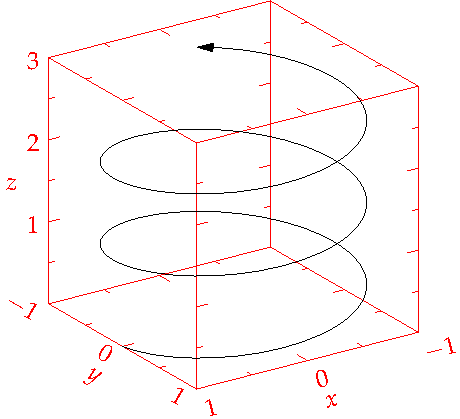
\includegraphics[width=\linewidth]{helix}
  \caption{This is a margin figure.  The helix is defined by 
    $x = \cos(2\pi z)$, $y = \sin(2\pi z)$, and $z = [0, 2.7]$.  The figure was
    drawn using Asymptote (\url{http://asymptote.sf.net/}).}
  \label{fig:marginfig}
\end{marginfigure}

\begin{docspec}
\textbackslash begin\{marginfigure\}\\
  \qquad\textbackslash includegraphics\{helix\}\\
  \qquad\textbackslash caption\{This is a margin figure.\}\\
  \qquad\textbackslash label\{fig:marginfig\}\\
\textbackslash end\{marginfigure\}\\
\end{docspec}

The \docenv{marginfigure} and \docenv{margintable} environments accept an optional parameter \docopt{offset} that adjusts the vertical position of the figure or table.  See the ``\nameref{sec:sidenotes}'' section above for examples.  The specifications are:
\begin{docspec}
  \textbackslash{begin\{marginfigure\}[\docopt{offset}]}\\
  \qquad\ldots\\
  \textbackslash{end\{marginfigure\}}\\
  \mbox{}\\
  \textbackslash{begin\{margintable\}[\docopt{offset}]}\\
  \qquad\ldots\\
  \textbackslash{end\{margintable\}}\\
\end{docspec}

Figure~\ref{fig:fullfig} is an example of the \docenv{figure*}
environment and figure~\ref{fig:textfig} is an example of the normal
\docenv{figure} environment.

\begin{figure*}[h]
  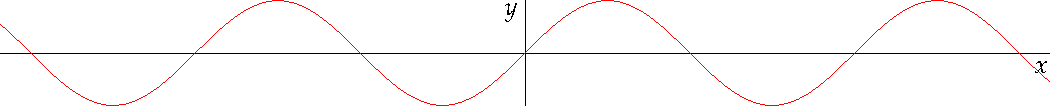
\includegraphics[width=\linewidth]{sine.pdf}%
  \caption{This graph shows $y = \sin x$ from about $x = [-10, 10]$.
  \emph{Notice that this figure takes up the full page width.}}%
  \label{fig:fullfig}%
\end{figure*}

\begin{figure}
  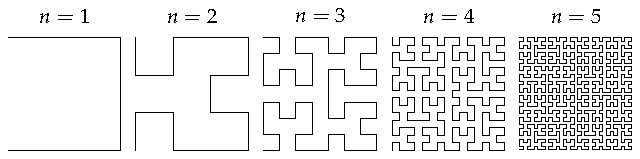
\includegraphics{hilbertcurves.pdf}
%  \checkparity This is an \pageparity\ page.%
  \caption[Hilbert curves of various degrees $n$.][6pt]{Hilbert curves of various degrees $n$. \emph{Notice that this figure only takes up the main textblock width.}}
  \label{fig:textfig}
  %\zsavepos{pos:textfig}
\end{figure}

\chapter{Conclusion}


%%
% The back matter contains appendices, bibliographies, indices, glossaries, etc.







\backmatter

\bibliography{biblio}
\bibliographystyle{apalike}


\printindex

\end{document}

